\documentclass{article}
\usepackage{importer}

\usepackage[backend=biber]{biblatex}
\addbibresource{kilder.bib}

\title{Forelesningsnotater: Faste Stoffers Fysikk}
\author{Sebastian Siljuholtet Johansen }
\date{Vår 2024}

\begin{document}

\maketitle

\nyside
\section*{Ingress}
Skrevet av studenter. Notater er tatt under forelesningene i TFY4220 Faste Stoffers Fysikk av Dag Werner Breiby. I tillegg har visse deler blitt utdypet og ekstra forklaringer har blitt lagt til visse deler.
\nyside
\tableofcontents

\nyside
\kapittel{Kapittel I: }
Hvordan atomer er ordnet kalles for \enquote{struktur}. Denne strukturen bestemmer egneskapene til et materiale. Altså hvordan det oppfører seg.

Vi diskuterer to slike typer av krystallinske materialer:
\begin{itemize}
    \item Amorfisk (glass, væsker, ...): som betyr tilfeldig.
    \item Krystallinske: som betyr periodisk i rom (i realiteten finnes det defekter).
\end{itemize}
Av disse krystallinske materialene har vi to typer:
\begin{itemize}
    \item Enkeltkrystaller: Som betyr at de har en uniform struktur.
    \item Polykrystaller: Disse er bygd opp av flere ulike periodiske strukturer i et materiale. På en måte en slags kobling av flere enkeltkrystaller. Hver enkelt av disse delene kalles for ulike korn. 
\end{itemize}
En tegning av disse er:
\begin{figure}[H]
    \centering
    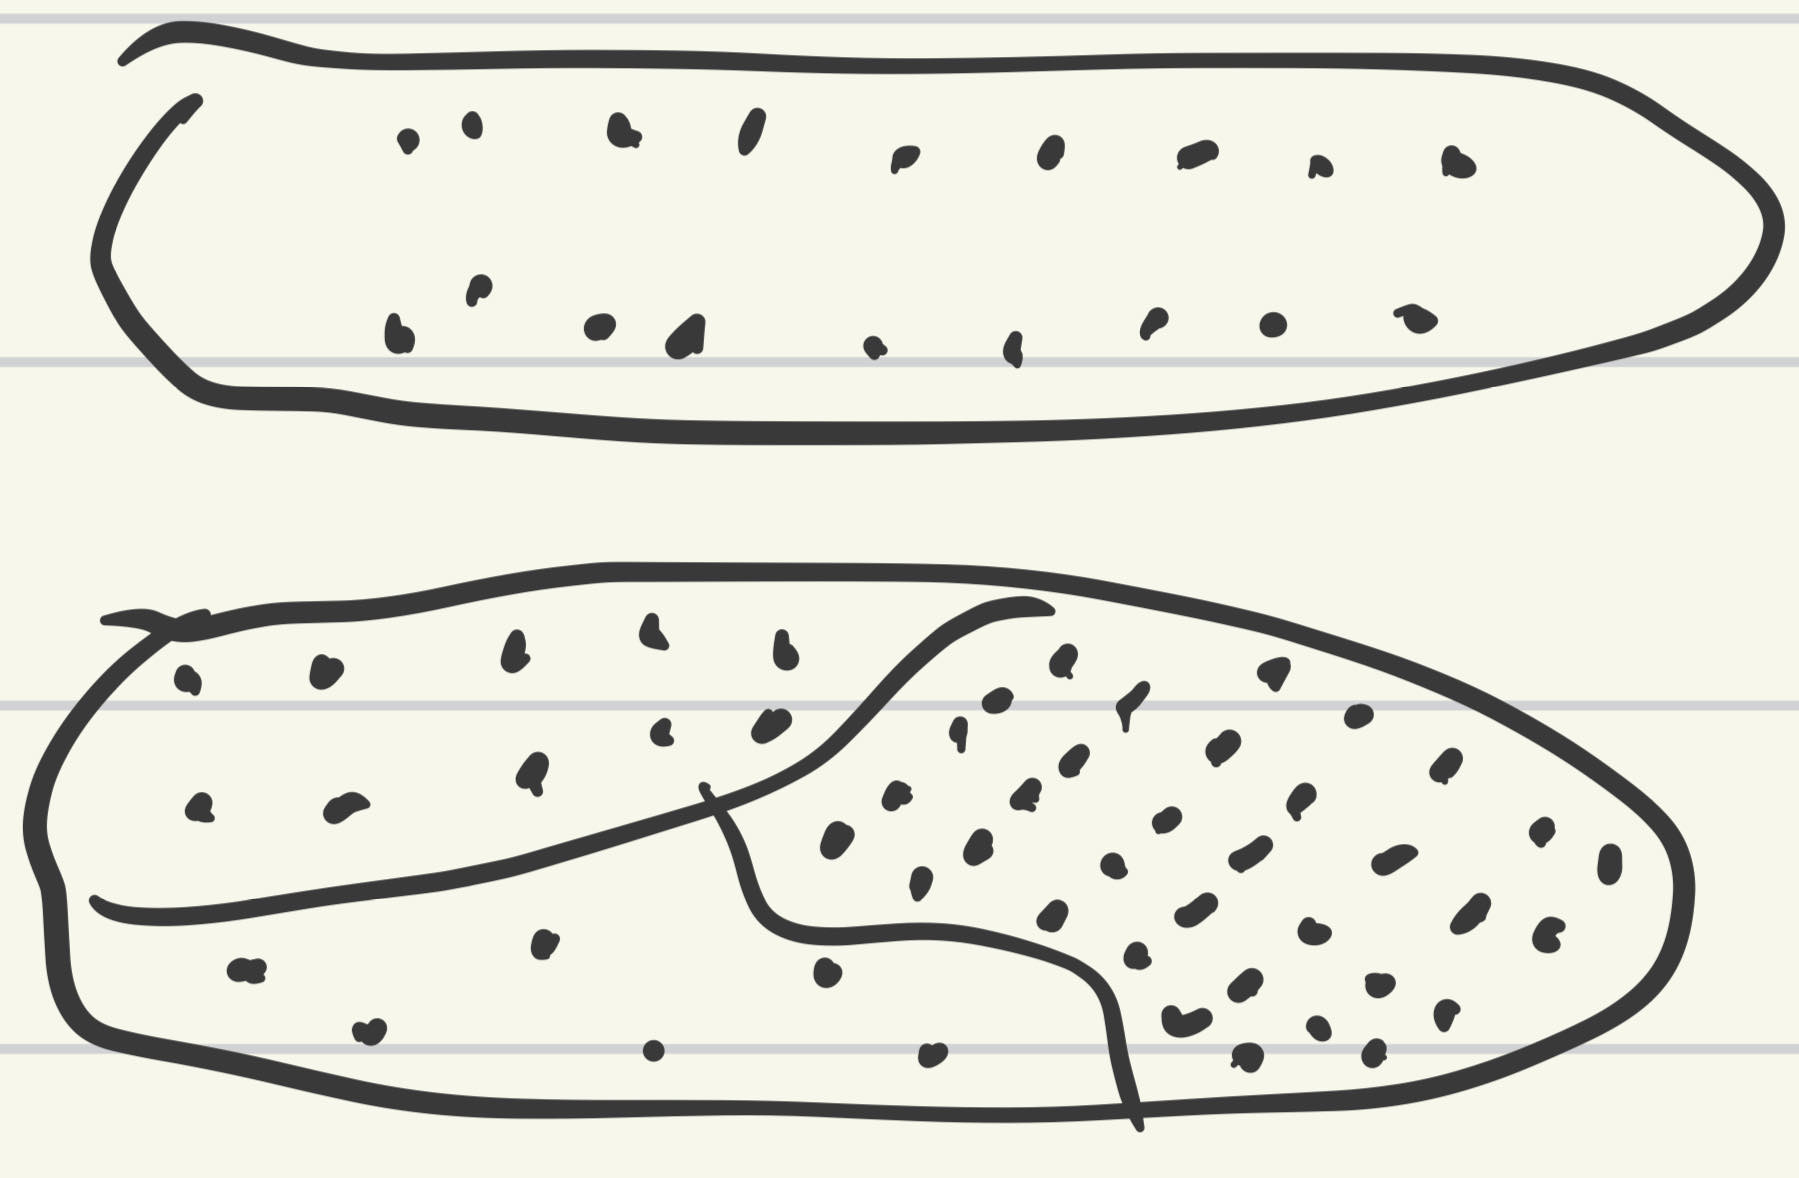
\includegraphics[width=0.5\linewidth]{bilder/enkelt_poly_krystaller.png}
    \caption{Enkelt krystall(over) og poly-krystall(under)}
    \label{fig:enkelt_poly_krystaller}
\end{figure}
I disse enkeltkrystallene har vi en eller annen translasjonell symmetri i domenet deres. Slik som en rotasjon, en speiling eller rene translasjoner.
\delkapittel{Bravais Gitter}
Et slikt gitter er bygd opp av en uendelig mengde med punkter som ser likt ut fra hvert eneste punkt. I en viss dimensjon d kan vi definere ethvert slikt punkt som:
\begin{align}
    \vec{R} = \sum_{i} n_i \vec{a}_i
\end{align}
I 2 dimensjoner finnes det kun 5 gyldige Bravais-gittere som alle er repeterende versjoner av 5 ulike figurer. Disse er repeterende firkant-, rektangulært-, heksagonalt-, sentrert-rektangulært og skråmønstere. Videre finnes det i 3 dimensjoner:
\begin{itemize}
    \item Triklinisk: $a\ne b\ne c$, $\alpha \ne \beta \ne \gamma \ne 90$ = 3D prisme
    \item Monoklinisk: $a \ne b \ne c$, $\beta \ne 90$, $\alpha = \gamma = 90$
    \item Ortorombisk: $a \ne b \ne c$, $\alpha = \beta = \gamma = 90$
    \item Tetragonalt: $a = b \ne c$, $\alpha = \beta = \gamma = 90$
    \item Kubisk: $a = b = c$, $\alpha = \beta = \gamma$. Dette er det vi vil se på.
\end{itemize}
Totalt finnes det 14 stykker av disse.
\seksjon{Kubiske systemer}
Det finnes tre forskjellige kubiske systemer. Disse kan tegnes som under \cite{kubiske_systemer}:
\begin{figure}[H]
  \centering
  \begin{subfigure}{0.3\textwidth}
    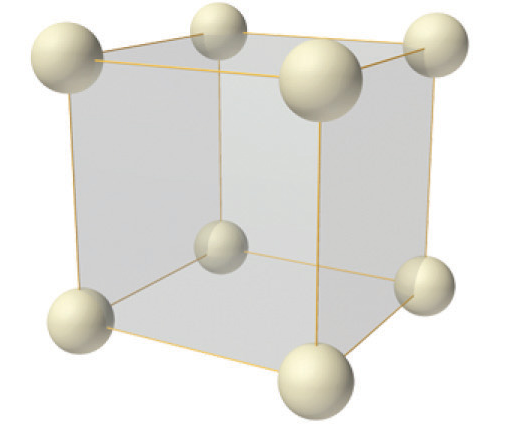
\includegraphics[width=\linewidth]{bilder/enkelt_kubisk.png}
    \caption{Enkelt kubisk (S.C)}
    \label{fig:enkelt_kubisk}
  \end{subfigure}
  \begin{subfigure}{0.3\textwidth}
    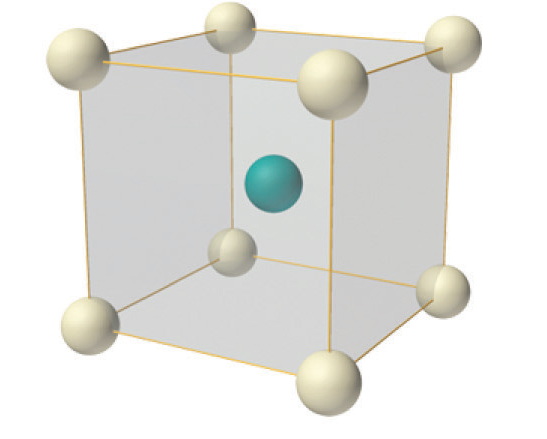
\includegraphics[width=\linewidth]{bilder/romsentert_kubisk.png}
    \caption{Romsentrert kubisk (B.C.C)}
    \label{fig:romsentert_kubisk}
  \end{subfigure}
  \begin{subfigure}{0.3\textwidth}
    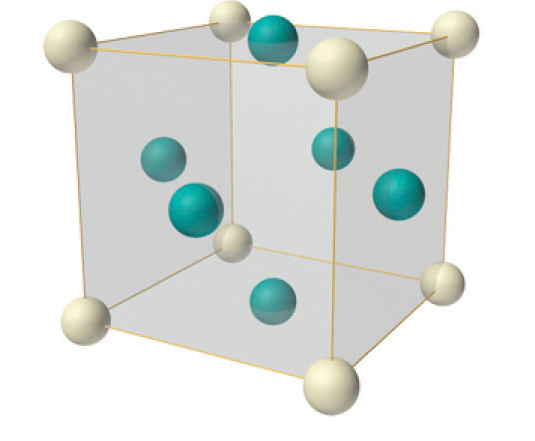
\includegraphics[width=\linewidth]{bilder/flatesentrert_kubisk.png}
    \caption{Flatesentrert kubisk (F.C.C)}
    \label{fig:flatesentrert_kubisk}
  \end{subfigure}
  \caption{Forskjellige typer kubiske systemer}
  \label{fig:kubiske_interpolasjoner}
\end{figure}
\seksjon{Enhetsceller}
Enhetsceller er byggeblokker. De kan for eksempel være prismer. De er da parameterisert av 6 tall. De tre lengdene som skaper et prisme og vinklene mellom den. Vi kaller en slik enhetscelle som kun inneholder ett Bravais-gitterpunkt for en primitiv enhetscelle. En enhetscelle har også som et krav at de må fylle alt av rommet nøyaktig hvis de blir flyttet og kopiert over alt rundt på Bravais-gitteret.
\seksjon{Wigner-Seiz-celle}
Et spesifikt valg av en slik enhetscelle er den hvor cellen er definert som alt volumet rundt et gitterpunkt som er nærmere det punktet enn alle de andre punktene. I et 2-dimensjonalt-firkantgitter vil disse enhetscellene kun bli en firkant rundt punktet med like lengder som firkantgitteret.
\seksjon{Basis}
Alle krystallstrukturer kan bli uttrykt som konvolusjonen mellom et Bravais-gitter med en \enquote{basis}. For eksempel ville vi kunne skrevet noe som $\dots \otimes O = O O O$. En grov illustrasjon av et faktisk gitter er Perovskitt. Dette er en struktur som består av et enkeltgitter, med en basis bestående av et atom A, et atom B og tre oksygen-atomer $O_3$. Stoffet er da (ABO3) generelt, men for Perovskitt er dette (BaTiO3). Dette illustreres grovt slik:
\begin{figure}[H]
    \centering
    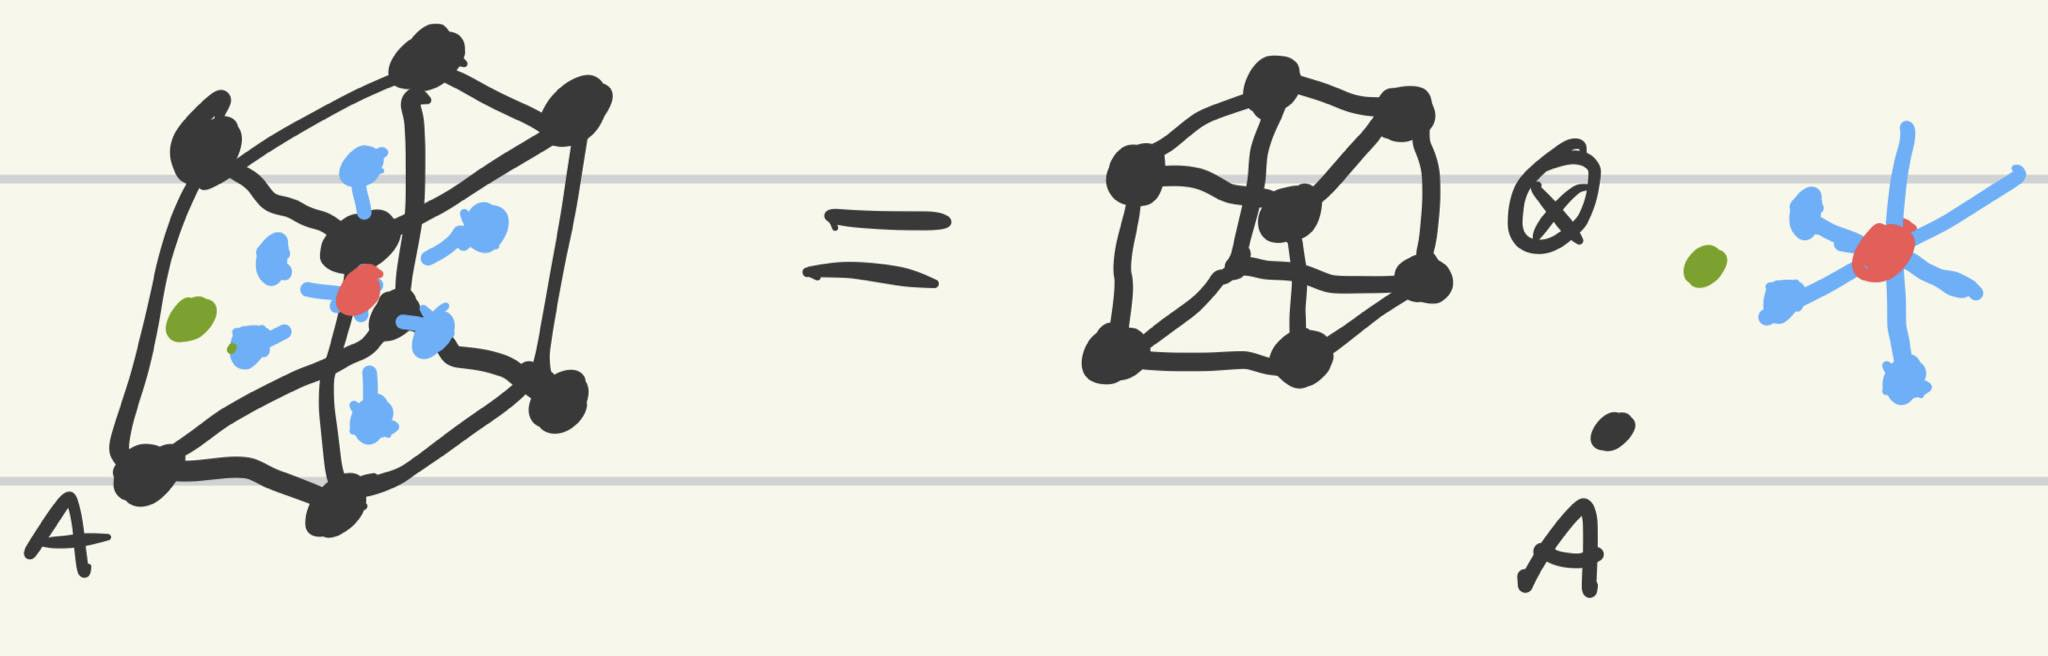
\includegraphics[width=0.5\linewidth]{bilder/perovskitt_gitter.png}
    \caption{Perovskitt-gitter (ABO3)}
    \label{fig:perovskitt_gitter}
\end{figure}
\seksjon{Fyllefaktor $\Phi$}
Et sentralt spørsmål for slike gittere vi snakker om er; hvor mye av rommet vil strukturen fylle, ved antagelsen av at atomene er sfæriske og tett pakket. For et enkeltgitter er dette: $\Phi_{S.C} \sim 52\%$. Derimot finnes det kun to naturlige stoffer som skaper en slik struktur: Fluorid og oksygen.

For et romsentrert kubisk struktur er fyllefaktoren en del høyere:$\Phi_{B.C.C} \sim 68\%$
\delseksjon{Tettpakking av sfærer}
F.C.C og heksagonalt-tettpakning (H.C.P) har den høyeste fyllefaktoren: $\Phi \sim 74\%$. Av grunnstoffene skaper 24 av dem et gitter i F.C.C-form og 36 i H.C.P-form.
\seksjon{Gitterplan}
Gitterplan er alle plan som inneholder minst 3 ikke-kolineære gitterpunkter. Altså er de plan som skapes i rommet ditt av en viss mengde punkter (langs ortonormale akser). I 3D, blir dette som skrevet over 3. De blir beskrevet av \underline{Miller-indekser}.
\delseksjon{Miller-indekser}
Hvis vi tar for oss 3D-rom vil vi få et koordinatsystem med 3 punkter langs aksene våre. Lengden til hver av disse 3 punktene som skaper planet kaller vi for $x_1, x_2, x_3$. VI definerer da at: $h = \frac{1}{x_1}, k = \frac{1}{x_2},l = \frac{1}{x_3}$. Dette er miller-indeksene. Vi kan for eksempel ha (100) som forteller oss at vi har et plan på $x_1$ = 1, mens $x_2, x_3 = \infty$.

\delseksjon{Gitterplan-familier}
Et annet tett knyttet tema er gitterplanfamilier. Ved å skyve et plan langs normalvektoren dens, vil man skape en familie av plan (i 2d blir det en familie av uendelig lange linjer).

Vi kaller nå avstanden mellom gitterplan som er plassert på ulike gitterpunkt for d-mellomrommet. Man kan vise at for ortoromber(som inneholder kuber) så har man at
\begin{equation}
    \frac{1}{d^{2}_{hkl}} = \frac{h^2}{a^2} + \frac{k^2}{b^2} + \frac{l^2}{c^2}
\end{equation}

Et viktig faktum å merke seg er at man kan bare ha 1, 2, 3, 4 og 6-foldige rotiasjoner av et gitter og fortsatt ha translasjonell symmetri. Med $n$-foldig mener jeg da  $360 / n$-graders-rotasjoner
\nyside
\kapittel{Kapittel II: Bølgediffraskjon og det Resiprokale Gitteret}
\delkapittel{Diffraksjon}
La oss først snakke om  hva slags typer diffraksjon vi har. Mer spesifikt, hva om skaper \underline{diffraksjon}:
\begin{itemize}
    \item Lys-mikroskop: Slike mikroskop ser på synlig lys. Altså er $\lambda \in (400, 600)$ nm. Her er også diffraksjonen begrenset av en oppløsning $\sim \frac{\lambda}{2}$
    \item Røntgenbølger: Disse har energi tilsvarende $\sim 10 $keV, $\lambda \sim 1.5$Å
    \item Elektron-mikroskop: Slike mikroskop ser på elektroner. Disse har en energi tilsvarende $\sim 20 keV$, $\lambda << 1$Å.
    \item Nøytroner: Disse er nøytrale partikler som oppfører seg som De Broglie-materiebølger og vekselvirker med atomkjernens magnetiske strukturer.
\end{itemize}
La oss se vekk fra linser og mikroskopi. Vi vil se på diffraksjon på periodiske krystaller.
\seksjon{Bragg's lov}
\begin{wrapfigure}{r}{0.4\textwidth}
    \centering
    \fbox{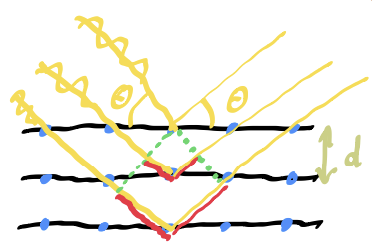
\includegraphics[width=0.4\textwidth]{bilder/braggs_lov.png}}
    \caption{Bragg's lov}
    \label{fig:braggs_lov}
\end{wrapfigure}
Betrakt atomplan som reflekterende speil. Bølgende skaper en konstruktiv interferens i disse atomplanene når $n \lambda = 2d \sin(\theta)$. En illustrasjon av hva som skjer er til høyre i \ref{fig:braggs_lov}. Her har vi innkommende bølger fra venstre som beveger seg vekk igjen etter å ha blitt speilet, med samme vinkel som de kom inn. Atomplanene er da linjene som skapes mellom ved hvert plan. Lengden mellom disse er da $d$ og er de samme lengdene som d-mellomrommet. Hvis man da vet Miller-indeksene til et type gitter og hva slags gitter det er, kan man finne ut hvordan diffraksjon vil foregå. Ofte i motsatt reggefølge for å finne ut et stoff.
\seksjon{Rayleigh-Spredning}
Rayleigh-spredning er en type spredning som forekommer ved elastisk spredning av fotoner av materie. Vi har derfor energi og impulsbevaring, og da bevaring av bølgelengden til fotonene. Altså har vi følgende:
\begin{itemize}
    \item Energi og impulsbevaring
    \item $\Rightarrow \lambda_i = \lambda_0$
    \item Videre har vi: $\Rightarrow k = |\vec{k}_1|= |\vec{k}_p| = \frac{2 \pi}{\lambda}$
\end{itemize}
En illustrasjon av spredningen kan se slik ut \ref{fig:rayleigh_spredning}:
\begin{figure}[H]
    \centering
    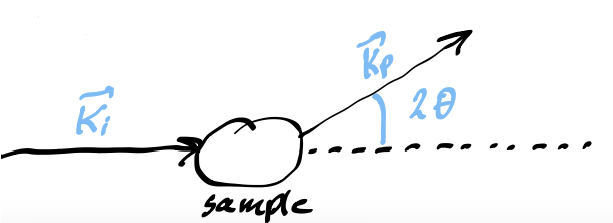
\includegraphics[width=0.3\textwidth]{bilder/rayleigh_spredning.png}
    \caption{Rayleigh spredning}
    \label{fig:rayleigh_spredning}
\end{figure}

Rayleighs lov er da at:
\begin{equation}
\label{eq:rayleighs_lov}
\text{Sprednings-styrke} \propto \frac{1}{\lambda^4}
\end{equation}
Dette fører for eksempel til at vi ser blått lys i himmelen og rødt ved en solnedgang. De minste bølgelengdene blir spredt først og de lengste sist.

\seksjon{Kinematisk Diffraksjonteori}
For å se litt nøyere på diffraksjon tar vi for oss kinematikken bak det. La oss anta at vi har en enkelt spredningshendelse. Vi har elastisk Rayleigh-spredning med en spredningsvektor definert som $\vec{Q} \defeq \vec{k}_f - \vec{k}_i$ og $|\vec{Q}| = \frac{4\pi}{\lambda} \sin(\theta)$. Dette blir faseforskjellen til bølgene. Når vi har et momentum $k_i$ før og $k_f$ etter og bølgene ser ut som $\propto e^{i \vec{k} \cdot \vec{r}}$, vil faseforskjellen bli til $e^{-i \vec{Q} \cdot \vec{r}}$. Spredningen som kommer fra et lite volumelement i en et gitter blir da noe som:
\begin{align}
    dF(\vec{Q}) = \underbrace{\rho(\vec{r})}_{\text{elektron-tetthet}} \underbrace{e^{-i \vec{Q} \cdot \vec{r}}}_{\text{fasefaktor}} dV
\end{align}
Her er F spredningsamplituden. Altså vil litt spredning avhenge av elektrontettheten ganger faseforskjellen til spredning i en retning $\vec{r}$. Totalt sett har vi:
\begin{align}
    F(\vec{Q}) = \int_{\text{prøven}} dV \rho(\vec{r})e^{-i \vec{Q} \cdot \vec{r}}
\end{align}
Her ser vi da at spredningsamplituden er fourier-transformen av elektrontettheten. Altså kan vi finne elektrontettheten ved å gjøre en invers-fouriertransform av spredningsamplituden.

Dessverre kan vi ikke måle F(Q). Det eneste vi kan måle er strålingsintensiteten: $I(\vec{Q}) \propto |F(\vec{Q})|^2$.

\delkapittel{Det Resiprokale Gitteret (Impulsrommet)}
Ved å gjøre en fourier-transformasjon kan vi komme til Impulsrommet ($\vec{r} \rightarrow \vec{Q}$. Her vil enhver vektor i det reelle rommet tilsvare noe lik inversen i impulsrommet. En lengde $d$ vil bli $d = \frac{2 \pi}{Q}$ hvor Q er lengden til en vektor i impulsrommet. For eksempel vil et gitter, bestående av deltafunksjoner, bli til en sum av planbølger i impulsrommet. Altså tilsvarer et punkt i det ene rommet, en bølge i det andre. Mer spesifikt og nyttig er at et punkt i impulsrommet, er en planbølge i posisjonsrommet med impulsen som tilsvarer det punktet i impulsrommet. Videre vil et slikt gitter, bestående av uendelig mange deltafunksjoner, bli til et nytt gitter i impulsrommet. Forskjellen her blir da at hvis dette gitteret har en gitterlengde på $a$, vil det i impulsrommet ha motsatt skalering med en faktor. I gitterrommet får vi at $a^{*} = \frac{2\pi}{a}$. Kort sagt:
\underline{Fouriertransformen av et gitter er ett nytt gitter}.

Videre må vi ha for det resiprokte gitteret at for gittervektorene: $e^{i \vec{G} \cdot \vec{R}} \Rightarrow \vec{G} \cdot \vec{R} = 2 \pi n$. For de gittervektorene vi har, har vi videre:
\begin{align}
    \vec{R}: \vec{R}_{mno} &= m \vec{a}_1 + n\vec{a}_2 + o \vec{a}_3 \text{  | Bravais-gitter} \\
\vec{G}: \vec{G}_{hkl} &= h \vec{a}^{*}_1 + k\vec{a}^{*}_2 + l\vec{a}^{*}_3 \text{  | Resiprokale-gittervektor} \\
\Rightarrow a_i^{*} &= 2 \pi \frac{\vec{a}_j \times \vec{a}_k}{\vec{a}_1 \cdot (\vec{a}_2 \times \vec{a}_3)} \varepsilon_{ijk} \\
\Rightarrow \vec{a}_i \cdot \vec{a}^{*}_{j} &= \delta_{ij} 2 \pi \\
\Rightarrow e^{i \vec{G} \cdot \vec{r}} &= e^{i \vec{G} \cdot \vec{r}} \\\cdot e^{i \vec{G} \cdot \vec{R}} &= e^{i \vec{G} \cdot(\vec{R} + \vec{r})}
\end{align}
Vi har dermed at enhver fysisk egenskap må ha periodisiteten til gitteret. Dette er \underline{veldig} viktig. Videre fra logikken utført over vil $\vec{R}$ definere Bravaisgitteret i posisjonsrommet, mens $\vec{G}$ definerer det samme Bravaisgitteret i impulsrommet. Et viktig teorem er at $d_{hkl} = \frac{2\pi}{|\vec{G}_{hkl}|}$

Vi kan dermed definere:
\begin{align}
    \text{Generell fourier-rekke: } n(\vec{r}) &= \sum_{\vec{q}} n_{\vec{q}} e^{i \vec{q} \cdot \vec{r}} \\
   \text{Periodisk fourier-rekke: } n(\vec{r}) &= \sum_{\vec{G}} n_{\vec{G}} e^{i \vec{G} \cdot \vec{r}} \\
\end{align}
Her vil vi jo da ha et mengden med periodiske elementer vil være en undermengde av alle fourierelementene. Altså $\{\vec{G}\} \in \{\vec{g}\}$
\seksjon{Spredning av et krystallgitter}
Vi har som sagt at:
\begin{equation}
    F(\vec{Q}) = \int \rho(\vec{r}) e^{-i \vec{Q} \cdot \vec{r}} dv \tab[2cm] I(\vec{Q}) \propto |F(\vec{Q})|^2
\end{equation}
På en atomisk skala vil $\rho(\vec{r})$ være diskret: $\int_{\text{prøve}} dV \rightarrow \sum_\alpha \underset{\text{krystallisk}}{\rightarrow} \underbrace{\sum_{u}}_{\text{enhetsceller}} \underbrace{\sum_{\alpha \in u}}_{\text{atomer i enhetscelle}}$.

Dette vil da gjøre om $F$ til:
\begin{equation}
    F(\vec{Q}) \rightarrow \sum_n \sum_j\underbrace{f_j(\vec{Q})}_{\substack{\text{Atom-formfaktoren.} \\ \text{Spredningsmulighet fra det j. atomet.} \\ \text{F.T av elektrontettheten på det j. atomet.}}} e^{-i\vec{Q}(\vec{R_n} + \vec{r_j})}
\end{equation}
Her kommer da $(\vec{R_n} + \vec{r_j})$ fra at $R$ tar oss til enhetscellen, mens $r$ tar oss til individuelle atomer i basisen rundt ved cellen. Denne likningen for F kan vi dele og den blir videre til:
\begin{equation}
    F(\vec{Q}) = \underbrace{\sum_n e^{-i \vec{Q} \cdot \vec{R}_n} }_{\text{Gittersum}}\cdot \underbrace{\sum_j e^{-i \vec{Q} \cdot \vec{r}_j}}_{\text{Strukturfaktor}}
\end{equation}
Her er det nyttig hvis vi ser på disse to delene, og hva som skjer her:

\begin{minipage}{0.45\textwidth}
\delseksjon{Enhetscell-Strukturfaktor}
Strukturfaktoren er som sagt definert som: \begin{equation}
    S = \sum_J f_j (Q) e^{-i \vec{Q} \cdot \vec{r}_j}
\end{equation}
Ved å da se på når gittersummen blir stor har vi at $\vec{Q} = \vec{G}$, som beskrevet til høyre. Videre blir da:
\begin{align}
    \vec{Q} \cdot \vec{r}_j &= (h \vec{a}^{*} + k \vec{b}^{*} + l \vec{c}^{*}) \cdot(x_J \vec{a} + y_j \vec{b} + z_j \vec{c}) \\
    &= 2 \pi (h x_j + ky_j + lz_j)
\end{align}
Altså har vi totalt sett at strukturfaktoren, når vi har sterkest diffraksjon blir:
\begin{equation}
\label{eq:strukturfaktoren}
    \boxed{S = \sum_j f_j(Q) e^{-i 2 \pi (h x_j + ky_j + lz_j)}}
\end{equation}
\end{minipage}
\hfill
\begin{minipage}{0.45\textwidth}
\delseksjon{Gittersummen}
Her kommer $n$ til å være enorm. I tillegg kommer summen av $n$ slike eksponenter mest sannsynlig til å gå mot 1 med mindre noe presser eksponentene til å bli noe annet enn en. Uansett vil vi få en veldig stor sum hvis $\vec{Q} \cdot \vec{R}_n = 2 \pi m$. Ellers vil summen gå mot 1. Dette er jo diffraksjonsbetingelsen og dermed er $\vec{Q} = \vec{G}$ når denne summen blir stor, og da altså når spredningsamplituden er stor.
\end{minipage}

\begin{tcolorbox}[breakable,boxrule=0pt]
  \delseksjon{Eksempel 1:}

    Vi har et FCC gitter med separasjon $a = 4.05$Å.

    Her må vi se på hvordan det ser ut i figur \ref{fig:fcc_enhets_celle}.     \begin{wrapfigure}{r}{0.4\textwidth}
        \centering
         \fbox{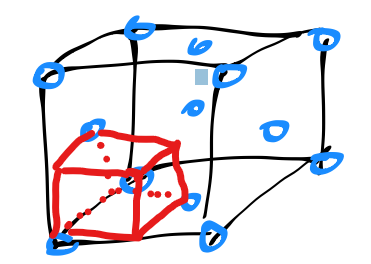
\includegraphics[width=0.4\textwidth]{bilder/fcc_enhets_celle.png}}
        \caption{FCC enhetscelle}
        \label{fig:fcc_enhets_celle}
    \end{wrapfigure}I denne figuren ser vi at den røde kuben inne i fcc-gitteret representerer enhetscellen vi bryr oss om. Her vil vi da summe over alle atomene som ikke er ekvivalente her. Siden posisjonene til de ytterste atomene er halvparten av hele fcc-gitteret får de posisjoner i enten x, y eller z som blir $1/2$. Posisjonene blir da: $(0,0,0), (\frac{1}{2}, \frac{1}{2}, 0), (\frac{1}{2}, 0, \frac{1}{2}), (0, \frac{1}{2}, \frac{1}{2})$. Vi får da for strukturformfaktoren:
    \begin{equation}
        S = f\left\{1 + e^{-i \pi(h+k)} + e^{-i \pi(h+l)} + e^{-i \pi(k+l)}\right\}
    \end{equation}
    Hvor vi har sagt at $f_j = f$ og dermed uavhengig av atom. Videre har vi ved å ta hensyn til at $h, k, l$ er heltall:
        \begin{equation}
        S = \Bigg\{ \substack{4f \tab[0.25cm]|\tab[0.25cm] h, k, l \text{ alle like/odde} \\ 0 \tab[0.25cm]|\tab[0.25cm] h,k,l \text{ ellers.      }}
    \end{equation}

\end{tcolorbox}

\begin{tcolorbox}[breakable,boxrule=0pt]
  \delseksjon{Eksempel 2:}

    Vi har et BCC gitter

    Her må vi se på hvordan det ser ut i figur \ref{fig:bcc_enhetscelle}.     \begin{wrapfigure}{r}{0.4\textwidth}
        \centering
         \fbox{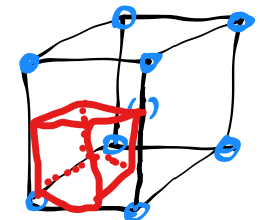
\includegraphics[width=0.4\textwidth]{bilder/bcc_enhetscelle.png}}
        \caption{BCC enhetscelle}
        \label{fig:bcc_enhetscelle}
    \end{wrapfigure}I denne figuren ser vi at den røde kuben inne i bcc-gitteret representerer enhetscellen vi bryr oss om. Her vil vi da summe over alle atomene som ikke er ekvivalente her. Siden posisjonene til det midterste atomet er halvparten av hele fcc-gitteret får den posisjoner i x, y eller z som blir $1/2$. Posisjonene blir da: $(0,0,0), (\frac{1}{2}, \frac{1}{2}, \frac{1}{2})$. Vi får da for strukturformfaktoren:
    \begin{equation}
        S = f\left\{1 + e^{-i \pi(h+k + l)}\right\}
    \end{equation}
    Hvor vi har sagt at $f_j = f$ og dermed uavhengig av atom. Videre har vi ved å ta hensyn til at $h, k, l$ er heltall:
        \begin{equation}
        S = \Bigg\{ \substack{2f \tab[0.25cm]|\tab[0.25cm] h+k+l \text{ like} \\ 0 \tab[0.25cm]|\tab[0.25cm] h+k+l \text{ odde}}
    \end{equation}
    Dermed har vi at: $I \propto |S(Q)|^2 = \Bigg\{ \substack{4f^2\\0}$

\end{tcolorbox}
\delseksjon{Atomformfaktoren}
I utrykket vårt for S (se \ref{eq:strukturfaktoren}) har vi størrelsen $f_j$, som er et mål av spredningskraften til det $j$. atomet i enhetscellen. Verdien inneholder antallet og spredningen til atomets elektroner, og bølgelengden og vinkelen av spredning til strålingen. La oss gjøre en klassisk utregning av denne. Først så må vi repetere hva den var definert som:
\begin{equation}
    \label{eq:atomformfaktoren}
    f_j = \int dV n_j(\vec{r}) e^{-i \vec{G} \cdot \vec{r}}
\end{equation}
Her går integralet over elektronfordelingen til et atom. La $\vec{r}$ ha en vinkel $\alpha$ med $\vec{G}$. Altså: $\vec{G} \cdot \vec{r} = G r \cos(\alpha)$. Hvis elektronfordelingen nå er sfærisk symmetrisk rundt origo så har vi:
\begin{align}
    f_j &= \int dV n_j(\vec{r}) e^{-i \vec{G} \cdot \vec{r}} \\
    &= 2 \pi \int dr r^2 d(\cos(\alpha)) n_j(r) e^{- i G r \cos(\alpha)} \\
    &= 2 \pi \int dr r^2 n_j(r) \cdot \frac{e^{iGr} - e^{-iGr}}{iGr} \eqexplain{Her går $\cos(\alpha)$ fra $-1$ til $1$}\\
    &= 4 \pi \int dr n_j(r) r^2 = \frac{\sin(Gr)}{Gr}
\end{align}
Hvis nå, elektrontettheten var veldig konsentrert rundt r som vi ofte har, vil vi få at denne sinusfaktoren blir lik 1. Da får vi at $f_j$ kun blir integralet over elektrontettheten og dermed blir $f_Jj = Z$ som er et svært viktig resultat:
\begin{equation}
\label{eq:atomformfaktor_lik_z}
    \boxed{f_j = 4 \pi \int dr n_j(r) r^2 = Z}
\end{equation}
\seksjon{Brillouin-sonen}
Briolouinsonen er definert av en Wigner-Seitz primitiv celle i impulsromgitteret. Denne sonen, innheolder alle bølgevektorer $\vec{k}$ som kan bli Bragg-refklektert av en krystall. La meg derfor komme med en mer rigorøs måte å skape en Wigner-Seitz-celle
\delseksjon{Å lage en Wigner-Seitz celle}
En primvitiv celle kan bli laget ved å følge denne prosedyren:
\begin{enumerate}
    \item Tegn ligner mellom et gitterpunkt og alle dets nærliggende gitterpunkter.
    \item På midtpunktet av disse linjene mellom gitterpunktene lager vi et plan/linje som er normal på linja som utvider seg utover.
    \item Det minste volumet rundt det originale gitterpunktet som er skapt av disse planene skaper da den primitive wigner-seitz-cellen.
\end{enumerate}

\nyside
\kapittel{Kapittel III: Krystallbindinger og Elastiske konstanter}
\delkapittel{Leonard-Jones Potensialet}
\begin{wrapfigure}{r}{0.25\textwidth}
    \centering
    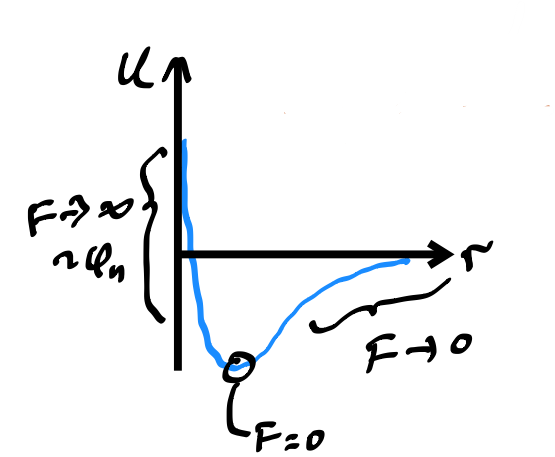
\includegraphics[width=0.25\textwidth]{bilder/leonard_jones_potensialet.png}
    \caption{Leonard-Jones Potensialet}
    \label{fig:leonard_jones_potensialet}
\end{wrapfigure}
Vi har mange ulike situasjoner inne i atomer, men den første vi skal ta for oss er at vi har Leonard-Jones potensialet. Her har vi et potensial som ser ut som i figuren til høyre \ref{fig:leonard_jones_potensialet}. Mattematisk ser det slik ut:
\begin{equation}
    \label{eq:leonard_jones_potensialet}
    u_{lj} \propto \frac{A}{r^{12}} - \frac{B}{r^6}
\end{equation}
Her skaper $r^6$ en Van der Waals vekselvirkning. Også kjent som London-vekselvirkningeen eller den induserte dipol-dipol vekselvirkningen. Det er hoved-tiltrekningskraften i krystaller av ikke-reagerende gasserr og i krystaller av mange organiske molekyler. Vekselvirkningen er en kvanteeffekt siden konstanten her vil avhenge av $\hbar$ og vil dermed forsvinne når vi tar grensen $\hbar \rightarrow 0$. Den vil også avhenge av $\alpha$ som er den elektroniske polariserbarheten.

Videre skaper $r^{12}$ faktoren, kreftene forårsaket av Pauli's utelukkelsesprinsipp. Dette prinsippet går ut på at to fermioner ikke kan overlappe helt. Altså kan de ikke ha helt like kvantetall. Dette er i motsetning til bosoner. På grunn av dette vil det skapes en effektiv kraft mellom elektroner som holder dem unna hverandre som vil ha et potensial i form av $\frac{A}{r^{12}}$.

Dette potensialet kan bli tilnærmet i mange av punktene, men spesielt ved $F = 0$ vil vi kunne tilnærme hele modellen som et harmonisk potensial og dermed som en fjær. Vi vil derfor kunne svingninger mellom atomer.

Typisk skriver man også om Van der Waals potensialet til:
\begin{equation}
    \label{eq:leonard_jones_potensialet_omskrevet}
    U(R) = 4 \epsilon \left[\left( \frac{\sigma}{R}\right)^{12} - \left( \frac{\sigma}{R}\right)^6 \right]
\end{equation}
Her er som normalt kreftene funnet av $F = -\frac{dU}{dR}$.
\seksjon{Gitterkonstantene ved Likevekt}
Hvis vi forkaster den kinetiske energien til atomene i den ikkereagerende gassen, vil den sammenhengende energien til en slik gaskrystall være gitt av å summe over alle par av atomer i krystallen. Hvis det er N atomer i krystallen blir da deres potensielle energi:
\begin{equation}
    U_{\text{tot}} = \frac{1}{2} N (4 \epsilon) \left[ \sum_j \left( \frac{\sigma}{p_{ij} R}\right)^{12} - \sum_j \left( \frac{\sigma}{p_{ij} R}\right)^6 \right]
\end{equation}
Her er $p_{ij} R$ avstanden mellom et referanseatom $i$ og alle andre atomer $j$, uttrykket i form av den næreste nabo-avstanden $R$. Faktoren $\frac{1}{2}$ kommer av at vi teller antall par dobbelt. For fcc-strukturen er summene over regnet ut til:
\begin{align}
    \sum_j p_{ij}^{-12} = 12.13188 \tab[2cm] \sum_j p_{ij}^{-6} = 14.45392
\end{align}
Mens for hcp-strukturen har vi:
\begin{align}
    \sum_j p_{ij}^{-12} = 12.13229 \tab[2cm] \sum_j p_{ij}^{-6} = 14.45489
\end{align}
Hvis vi nå hadde funnet likevektsavstanden for disse to strukturene (som er veldig like), må vi sette kraften lik null. Da får vi at:
\begin{equation}
\frac{R_0}{\sigma} = 1.09
\end{equation}
De observerte og målte verdiene til ulike stoffer er svært likt dette. For Ne (1.14), Ar(1.11), Kr(1.10) og Xe(1.09). Dette er kjempenærme og veldig merkverdig. De små forskjellene kommer av nullpunkt-kvanteeffekter.
\seksjon{Den Sammenhengende Energien}
Den sammenhengende energien til ikkereagerende gaskrystaller ved det absolutte nullpunkt og ved null trykk er funnet ved å sette inn $R_0$ i Leonard-Jones potensialet. Da får vi at:
\begin{equation}
    U_{\text{tot}}(R_0) = - (2.15) (4 N\epsilon)
\end{equation}
Dette er da det samme for alle slike gassser og er den utregnede sammenhengende energien når atomene er i likevekt. Kvantemekaniske korreksjoner vil redusere bindingsenergien med opptil 30\% for de nevnte stoffene over. Mest for Ne(28\%)

Jo tyngre atomet er, jo mindre er kvantekorreksjonene.

\delkapittel{Ioniske Krystaller}
Ioniske krystaller er bygget opp av positive og negative ioner Det ioniske båndet har sitt opphav i de elektrostatiske vekselvirkningene til motsatt ladde ioner. To vanlig krystallstrukturer for slike ioniske krystaller er krystallstrukturene til salt og cesium-klorid som består av et FCC-gitter med en basis som har ett atom i seg over det normale gitteret. 

\seksjon{Elektrostatiske/Madelung- Energien}
Den langtvirkende vekselvirkningen mellom motsatt ladde ioner er Coulomb-vekselvirkningen $\pm \frac{q^2}{r}$. Selv om vi har snakket om Van der Waals-krefter er det ikke de som skaper mesteparten av den sammenhengende energien i ioniske krystaller. Det er faktisk bare 1 til 2\% av energien som kommer av slike krefter. Merparten kommer fra elektrostatiske krefter og kalles for \underline{Madelung energien}.

Hvis $U_{ij}$ er vekselvirkningsenergien mellom ion $i$ og ion $j$ kan vi definere en energi som inneholder alle vekselvirkninger med et ion som:
\begin{equation}
    U_i = \sum_j U_{ij}
\end{equation}
Vi antar at $U_{ij}$ kan bli skrevet som summen av et sentralt frastøtende felt i formen $\lambda e^{-\frac{r}{\rho}}$, og et Coulomb-potensiale $\pm \frac{q^2}{r}$:
\begin{equation}
    U_{ij} = \lambda e^{-\frac{r_{ij}}{\rho}}\pm \frac{q^2}{r_{ij}}
\end{equation}
Hvis vi nå igjen definerer $r_{ij} = p_{ij} R$ og bare tar med den frastøtende vekselvirkningen blant næreste-naboer har vi:
\begin{equation}
 U_{ij} = \Bigg \{
\begin{array}{c}
\lambda e^{- \frac{R}{\rho}} - \frac{q^2}{R} \text{ Næreste naboer}\\ 
\pm \frac{1}{p_{ij}}\frac{q^2}{R} \text{ ellers}
\end{array}
\end{equation}
Da får vi totalt med $N$ atomer og $z$ næreste naboer:
\begin{equation}
    U_{\text{tot}} = N U_i = N\left(z\lambda e^{-\frac{R}{\rho}} - \alpha\frac{q^2}{R}\right)
\end{equation}
Hvor vi her har definert det vi kaller for \underline{Madelung konstanten}:
\begin{equation}
    \label{eq:madelung_konstant}
    \alpha \defeq = \sum_j \frac{\pm}{p_{ij}}
\end{equation}
Man kan også skrive om denne likningen for $U_{\text{tot}}$ i forhold til likevektsavstanden $R_0$. Da får man:
\begin{equation}
    U_{\text{tot}} = \underbrace{- \frac{N \alpha q^2}{R_0}}_{\defeq \text{Madelung-Energien}} \left(1 - \frac{\rho}{R_0}\right)
\end{equation}
Man kan også finne ut at $\rho \propto 0.1 R_0$ og dermed har denne frastøtende kraften veldig liten rekkevidde.
\seksjon{Utregning av Madelung-konstanten}
Ved å se på definisjonen av Madelung-konstanten kan vi bytte litt og få følgende formel:
\begin{equation}
    \frac{\alpha}{R} = \sum_j \frac{\pm}{r_j}
\end{equation}
Her får vi $+$ for positive ioner og $-$ for negative ioner. Man kan da bruke denne formelen hvis man kan avstanden til de næreste naboene i en krystall så har man $R$, og hvis man vet hvordan alle de andre avstandene er fra et referanseatom kan man sette inn disse for $r_j$ og regne ut $\alpha$.

\begin{tcolorbox}[breakable,boxrule=0pt]
    \delseksjon{Eksempel: Uendelig linje av alternerende ioner}
    La oss forestille oss at vi har en uendelig linje av alternerende ioner. Vi velger et negativt ion som referanseione og får derfor at:
    \begin{equation}
        \sum_j \frac{\pm}{r_j} = 2\left( \frac{1}{R} - \frac{1}{2R} + \frac{1}{3R} + \dots\right) = 2 \ln(2) / R
    \end{equation}
    Altså har vi:
    \begin{align}
        \frac{\alpha}{R} &= \frac{2\ln(2)}{R} \\
        \alpha &= 2 \ln(2)
    \end{align}
\end{tcolorbox}

\delkapittel{Kovalente Krystaller}
Den kovalente bindingen er det klassiske elektronpar eller den homopolare bindingen i kjemi. Spesielt i organisk kjemi. Det er en sterk binding. En slik kovalent binding er  typisk skapt av to elektroner, fra to forskjellige atomer. De pleier videre å være lokalisert i regionen mellom de to atomene som skaper bindingen. Spinnen til disse to elektronene er også antiparallelle.

Bindingen til molekylært hydrogen er et enkelt eksempel av en kovalent binding. Selv om bindingen kan skje med parallelle spinn er den sterkest med antiparallelle. Grunnen til at bindingen avhenger av dette er at det er ikke på grunn av sterke magnetisk dipolkrefter mellom elektronene, men på grunn av Pauli-prinsippet. Prinsippet vil endre ladningsfordelingen i atomene i forhold til spinn-orienteringen. Denne spinn-avhengige Coulombenergien kalles for bytte-vekselvirkning.

Pauli-prinsippet gir en sterk frastøtende vekselvirkning mellom atomer med fylte skall. Hvis de ikke er fylte, vil elektron-overlapp kunne skje uten eksitasjon av elektroner til høyenergi-tilstander. Da vil bindingene være kortere. Når de da ikke er fylte vil vi derfor få tiltrekkende krefter mellom dem som drar de sammen slik at elektrontilstandene som mangler blir delt mellom dem. Ser man på hydrogen, vil det faktum at enkelte hydrogenatomer kun har et atom i sitt ene orbital vise at det ikke er fylt opp. Man kan jo ha to elektroner i hver orbital. Altså vil to hydrogenatomer tiltrekkes og dele to elektroner for å få et fylt opp skall/orbital.
\delkapittel{Metaller}
Metaller er kjennetegnet av høy elektrisk ledningsevne, og et stort antall med elektroner i stoffet som er frie til å bevege seg rundt, ofte  en eller to per atom. Elektronene som kan bevege seg rundt kalles for ledningselektroner. Disse elektronene har sitt opphav i Valensbåndet og blir eksitert fra det gjennom eksterne elektriske potensialer. Altså spenninger. 

Noe å merke seg er at metaller pleier å krystallisere seg i ganske tettpakkede strukturer som hcp, fcc og bcc. Det i motsetning til krystaller som diamanter og liknende.

Videre kan det nevnes at:
\begin{itemize}
    \item Avstandene mellom atomer i alkali-metallene er relativt store fordi den kinetiske energien til ledningselektronene er lavere ved større inter-atomiske avstander. Dermed den overnevnte krystallstrukturen.
    \item I overgangsmetallene er det ekstra bindinger fra de indre elektronskallene. Dermed er disse metallene og metallene rett etterpå i den periodiske tabellen, kjennetegnet av høy bindingsenergi.
\end{itemize}
\delkapittel{Hydrogenbindinger}
Fordi nøytralt hydrogen kun har et elektron så burde det bare skape bindinger med ett annet atom. Derimot, har man målt at i visse forhold, vil man ha at hydrogen kan skape dobbeltbindinger og fungere som et slags bindingsledd mellom stoffer som F, O og N. Dette kalles for hydrogenbindinger.

Hydrogenbindinger er viktige deler av vekselvirkningen mellom vannmolekyler og er ansvarlige, sammen med elektrostatiske tiltrekninger, for elektriske dipolmomenter som gir fysiske egenskaper til vann og is. De er også viktige i visse ferroelektriske krystaller og i DNA.
\delkapittel{Atomiske størrelser}
Avstander mellom atomer i krystaller kan bli målt veldig nøyaktig av røntgendiffraksjon. Ofte til $1$ del i $10^5$. Kan vi si at den observerte avstanden mellom atomer kan bli delvis gitt til atom A og atom B? kan en definitiv mening bli gitt til radiusen av et atom eller et ion, uansett hvilken krystall de er i? Strengt talt er svaret nei. Ladningsfordelingen rundt et atom er ikke en ren sfærisk grense. Uansett er konseptet av en slik atomsk radius nyttig for å forutsi avstandene mellom atomer. Eksistensen og sannsynlige gitterkonstanter til faser som ikke har blitt laget enda kan bli forutsett fra de additive egenskapene til atomers radiuser. Videre kan elektronkonfigurasjonen til bestanddelene (atomene) i krystaller, bli forutsett av å sammenligne de målte og forutsatte gitterkonstantene.

Man lager derfor en mengde av selvkonsistente radiuser for ulike typer bindinger. Man regner da ut radiusene man hadde fått for de ulike bindingene man har i et krystall og legger disse sammen for å finne ut hva radiusen burde være. Motsatt vei kan man forutsi hva slags krefter som er viktige i et stoff ved å se hvor nær radiusen man har målt er til de bestemte radiusene til ulike krefter.
\nyside
\kapittel{Kapittel IV: Fononer: Krystallvibrasjoner}
Fononer er termiske vibrasjoner av atomer i gitteret. Leonard-Jones potensialet tilnærmet til andre orden (harmonisk oscillator) gir en god tilnærming til små oscillasjoner rundt likevektsposisjonen. Altså har vi harmoniske potensialer, godt tilnærmede av Hook's fjærer. Tidligere var bølgene våre kontinuerlige i formen $e^{ikx}$, mens nå er de kun definert på en diskret måte rundt gitterpunktene og den atomiske strukturen $|u|$. I og med at vi har noe som $e^{ika}$ vil vi kun ha at den første Brillouinsonen er relevant for momentumet. Dette er fordi alle verdier hvor $|ka| > \pi$ vil være til at vi får samme resultat. Altså er de eneste bølgelendene vi ser på som relevante, de som er i den første Brillouin-sonen definert av $k = \frac{\pi}{a} = \frac{2\pi}{\lambda} \Rightarrow \lambda = 2a$. De tilfellene vi da ser på som relevante er når $k$ er mindre ka og dermed når $\lambda \geq 2a$. Alle andre bølger vil føre til den samme informasjonen for en elastisk bølge i gitteret.

Dette med at alle bølger med kortere bølgelende vil være urelevante kan vi tegne på følgende måte:
\begin{figure}[H]
    \centering
    \includegraphics[width=0.5\linewidth]{bilder/overlappende_bølgelengder_1_sone.png}
    \caption{Overlappende informasjon i bølger}
    \label{fig:overlappende_bølgelengder_1_sone}
\end{figure}
Haer kan vi se at begge disse bølgende vil ha samme informasjon, men ha helt forskjellig bølgelengde. Noter derimot at elektromagnetiske bølger som røntgenbølger kan ha disse verdiene og fortsatt ha en fysisk mening i og med at de beveger seg gjennom områdene mellom atomene. For en elastisk diskret lokalisert bølge som vi har her vil denne informasjonen kun være overflødig og ikke ha noe mer fysisk mening.

\delkapittel{1D Monoatomisk kjede}
Hvis vi tar for oss en 1-dimensjonal monoatomisk kjede kan vi tegne den slik:
\begin{figure}[H]
    \centering
    \includegraphics[width=0.5\linewidth]{bilder/monoatomisk_fjær_kjede.png}
    \caption{1D Monoatomisk kjede}
    \label{fig:monoatomisk_fjær_kjede}
\end{figure}
Her kan vi kalle $u_n$ for forskyvingen fra likevektsposisjonene. Altså har vi to fo fjærer i dette scenarioet her. En mellom $n-1$ og $n$ og en mellom $n$ og $n+1$:
\begin{align}
    m\frac{d^2u_n}{dt^2} &= F_{n \leftrightarrow n-1} + F_{n \leftrightarrow n+1} \\
    &= -\gamma(u_n - u_{n-1}) -\gamma(u_n - u_{n+1}) \\
    &= -\gamma(2 u_n - u_{n-1} - u_{n+1})
\end{align}
Hvis vi nå antar at vi har en normal friforplantende bølge multiplisert med gitterposisjonene for å ha samme periodisitet som dem, får vi at:
\begin{align}
    u_n &= u e^{i(k a n - \omega t)} \\
    \Rightarrow \frac{d^2 u_n}{dt^2}  &= u -\omega^2 e^{i(k a n - \omega t)} \\
    u_{n\pm1} &= u e^{i (ka(n\pm1) - \omega t)}
\end{align}
Vi kan nå sette inn disse i kraftlikningen over. Da får v i:
\begin{align}
    -m\omega^2  u e^{i(k a n - \omega t)} ) &=-\gamma\left( 2 u e^{i(k a n - \omega t)} -u e^{i (ka(n+1) - \omega t)} - u e^{i (ka(n-1) - \omega t)}   \right)\\
    \Rightarrow -m \omega^2 &= -\gamma \left(2 - e{-ika} - e^{ika}\right) \\
    &=-\gamma \left(2 - 2 \cos(ka)\right)\\
    \Rightarrow \omega(k) &= \sqrt{\frac{2 \gamma\left(1 - \cos(ka)\right)}{m} }\\
    &= 2 \sqrt{\frac{\gamma}{m}}\left|\sin\left(\frac{ka}{2}\right)\right|
\end{align}
Vi får da spredningsrelasjonen:
\begin{equation}
    \label{eq:spredningsrelasjon_monoatomisk_kjede}
    \omega(k) =  \omega_{\text{maks}} \left|\sin\left(\frac{ka}{2}\right)\right| \tab[2cm] \omega_{\text{maks}} = 2 \sqrt{\frac{\gamma}{m}}
\end{equation}
Denne spredningsrelasjonen ser ut som følgende:
\begin{figure}[H]
    \centering
    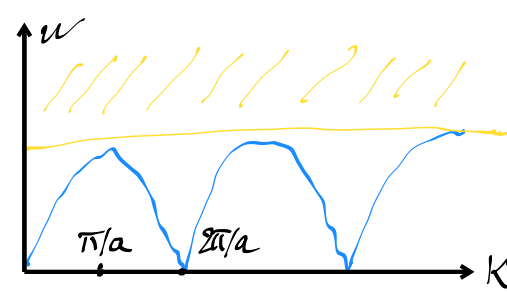
\includegraphics[width=0.5\linewidth]{bilder/spredningsrelasjon_fononer.png}
    \caption{Spredningsrelasjon for fononer}
    \label{fig:spredningsrelasjon_fononer}
\end{figure}
Her kan vi se at $\omega$ varierer mellom $0$ og $\omega_{\text{maks}}$ og er periodisk med $T = \frac{2\pi}{a} = \frac{4 \pi}{\lambda}$. Vi kan nå ta for oss to grenser. Når $\lambda$ er stor og $k \rightarrow 0$ og når $\lambda$ er så liten som mulig og dermed når $k \rightarrow \frac{\pi}{a}$. Altså midten eller kantene til den første Brillouinsonen.
\seksjon{Stor $\lambda$-grensen. Sentrum av Brillouin-sonen}
Her har vi da at $k \rightarrow 0$. På grunn av dette får vi at $\sin(\dots)$ kan bli tilnærmet i småvinkeltilnærmingen. Da har vi at:
\begin{equation}
    \omega(k) \approx \sqrt{ \frac{\gamma}{m}} ka \eqexplain{$\sin(x) \rightarrow x$}
\end{equation}
Vi har da at fasehastigheten vår blir: $\nu = \frac{\omega}{k}=a\sqrt{ \frac{\gamma}{m}} $.

Videre har vi at gruppehastigheten blir: $\nu_g = \frac{\partial \omega}{\partial k} = \nu$. Siden vi har at gruppehastigheten er det samme som fasehastigheten har vi \enquote{\underline{lydbølger}}. \\
\begin{wrapfigure}{r}{0.2\textwidth}
    \centering
    \fbox{\includegraphics[width=0.2\textwidth]{bilder/stående_bølge.png}}
    \label{fig:stående_bølge}
    \caption{Stående bølge}
\end{wrapfigure}
 \vspace{-1cm}
\seksjon{Små $\lambda$-grensen. Kanten av Brillouin-sonen}

Her har vi da at $\lambda \rightarrow 2a$. Da går $k \rightarrow k_{\text{maks}} = \frac{\pi}{a}$. Da får vi at:
\begin{equation}
    \omega(k) = a\sqrt{ \frac{\gamma}{m}} \eqexplain{$\sin(ka/2) \rightarrow \sin(\pi / 2) = 1$}
\end{equation}
Altså får vi en gruppehastighet: $\nu_g = \frac{\partial \omega}{\partial k} = 0$. 
Siden vi ikke har noen gruppehastighet, beveger ikke bølgen på seg og vi har dermed stående bølger. Dette kan tegnes som til høyre.

\seksjon{Estimering av Oscillasjonsamplituden}
Det kan være nyttig å se hvor sterk amplituden til disse fononene kan bli. Da tar vi først for oss hva energien vår er. Deretter kan vi sammenligne den potensielle energien og den potensielle energien for å så finne ut oscillasjonsamplituden:
\begin{equation}
    E = \frac{1}{2} mv^2 + \frac{1}{2} \gamma x^2
\end{equation}
Ekvipartisjonsteoremet sier at hvert kvadratisk ledd i energifunksjonen vil bidra med $\frac{1}{2} k_B T$ til den termiske energien. Altså får vi:
\begin{align}
    \frac{1}{2} \gamma x^2 = 2 * \frac{1}{2 } k_B T
\end{align}
Som gir oss at:
\begin{equation}
    x = \sqrt{\frac{2 k_B T}{\gamma}}
\end{equation}

\delkapittel{Spredningsrelasjonen i ulike tilfeller}
Videre kan det være nyttig å se litt tilbake på hvordan vi tidligere har sett på spredningsrelasjonene i andre tilfeller:
\seksjon{Frie partikler i kvantemekanikk}
For frie partikler i kvantemekanikk har vi følgende:
\begin{align}
    E = \hbar \omega = \frac{p^2}{2m} = \frac{\hbar^2 k^2}{2m}
\end{align}
Altså får vi følgende spredningsrelasjon:
\begin{equation}
    \label{eq:spredningsrelasjon_kvantemekanikk}
    \omega(k) = \frac{\hbar k^2}{2m}
\end{equation}
\seksjon{Lys i ulike stoffer}
Vi må også ta for oss lys i ulike stoffer. 
\delseksjon{Vakuum}
Først kan vi jo da nevne lys i vakuum. Da har vi at:
\begin{align}
    v\lambda &= c \\
    \Rightarrow \underbrace{(2\pi v)}_{= \omega} \underbrace{(\frac{\lambda}{2 \pi})}_{= 1/k} &= c \eqexplain{Gange med $\frac{2\pi}{2\pi}$}\\
    \Rightarrow \frac{\omega}{k} &= c
\end{align}
Altså har vi for lys i vakuum at:
\begin{equation}
    \label{eq:spredningsrelasjon_lys_i_vakuum}
    \omega(k) = ck
\end{equation}
\delseksjon{Andre medier}
I andre medier har vi en liten endring i forhold til lys i vakuum. Her vil faktisk \enquote{lysets hastighet} endre seg lokalt gjennom ulike stoffer og dermed på grunn av ulike spredningsprosesser bevege seg \enquote{tregere} gjennom hele materialet. Altså har vi noe vi kaller for refraksjonsindeksen $n > 1$:
\begin{equation}
    \label{eq:spredningsrelasjon_lys_i_medier}
    \omega(k) = k\frac{c}{n} = k c_{\text{medie}}
\end{equation}
\delkapittel{1D Diatomisk kjede}
En 1-dimensjonal diatomisk kjede kan bli tegnet på følgende måte:
\begin{figure}[H]
    \centering
    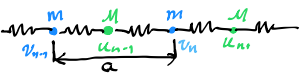
\includegraphics[width=0.5\linewidth]{bilder/diatomisk_kjede.png}
    \caption{Diatomisk Kjede}
    \label{fig:diatomisk_kjede}
\end{figure}
Her kan vi gjøre mye av det samme som vi gjorde for den monoatomiske kjeden. Vi må her derimot anta at vi har to forskjellige gitterstrukturer og derfor to likninger. En for den ene typen av atomer og en for den andre typen. Altså har vi en ansatz:
\begin{align}
    \label{eq:diatomisk_kjede_ansatz}
    u_n &= u e^{i (kan - \omega t)} \\
    v_n &= v e^{i (kan - \omega t)}
\end{align}
Vi må også ha to kraftlikninger. Vi har da ved å se på kjeden at vi har to forskjellige masser med forskjellige likninger for begge disse:
\begin{align}
    M \frac{d^2 u_n}{dt^2} &= F_{u_n \leftrightarrow v_n} + F_{u_n \leftrightarrow v_{n+1}}\\
                           &= -\gamma( u_n - v_n) -\gamma( u_n - v_{n+1}) \\
                           &= -\gamma(2u_n - v_{n} - v_{n+1}) \\
    m \frac{d^2 v_n}{dt^2} &= F_{v_n \leftrightarrow u_n} + F_{v_n \leftrightarrow u_{n-1}}\\
                           &= -\gamma( v_n - u_n) -\gamma( v_n - u_{n-1}) \\
                           &= -\gamma(2v_n - u_{n} - u_{n-1})
\end{align}
Vi kan nå sette inn likningene våre for $u_n$ og $v_n$ fra tidligere. Etter å ha satt inn dette vil vi kunne dele vekk flere av eksponentene men vil få noen cosinuser. La oss først ta for oss den første likningen så den andre:
\begin{align}
    M \frac{d^2 u_n}{dt^2} &= -\gamma(2u_n - v_{n} - v_{n+1})\\
    \Rightarrow M \omega^2 u e^{i(kan - \omega t)} &= \gamma\left(2 u e^{i(kan - \omega t)} - v e^{i(kan - \omega t)} - v e^{i(ka(n+1) - \omega t)}\right) \\
    \Rightarrow M \omega^2 u e^{i(kan)} &= \gamma\left(2 u e^{i(kan)} - v e^{i(kan)} - v e^{i(ka(n+1))}\right) \\
    \Rightarrow M \omega^2 u  &= \gamma\left(2 u - v  - v e^{i(kan)}\right) \\
    \Rightarrow 0 &= u (2 \gamma - M \omega^2) - v \gamma (1 + e^{i kan}) \\
\end{align}
Så har vi den andre likningen:
\begin{align}
    m \frac{d^2 v_n}{dt^2} &= -\gamma(2v_n - u_{n} - u_{n-1})\\
\Rightarrow m \omega^2 v e^{i(kan - \omega t)} &= \gamma\left(2 v e^{i(kan - \omega t)} - u e^{i(kan - \omega t)} - u e^{i(ka(n-1) - \omega t)}\right) \\
\Rightarrow m \omega^2 v e^{i(kan)} &= \gamma\left(2 v e^{i(kan)} - u e^{i(kan)} - u e^{i(ka(n-1))}\right) \\
\Rightarrow m \omega^2 v &= \gamma ( 2v - u - u e^{-ikan})\\
\Rightarrow 0 &= -u \gamma(1 + e^{-ikan}) + v (2\gamma - m \omega^2 )  
\end{align}
Altså har vi funnet et likningsett:
\begin{align}
    \label{eq:sprednings_relasjoner_diatomisk}
    u (2 \gamma - M \omega^2) - v \gamma (1 + e^{i kan}) &= 0\\
    -u \gamma(1 + e^{-ikan}) + v (2\gamma - m \omega^2 )  &= 0 
\end{align}
Disse kan bli omskrevet i matriseform ( vi har ganget med -1 også):
\begin{equation}
    \label{eq:sprednings_relasjoner_matrise_diatomisk}
    \twomatrix{ M \omega^2 - 2 \gamma }{\gamma  + \gamma e^{i kan}}{\gamma + \gamma e^{-i kan}}{ m \omega^2 - 2\gamma } \twovec{u}{v} = 0
\end{equation}
For at denne matrisen skal kunne løses må determinanten bli null. Da får vi:
\begin{align}
    & ( M \omega^2-2 \gamma ) \cdot ( m \omega^2 - 2\gamma) - (\gamma + \gamma e^{i kan}) \cdot (\gamma + \gamma e^{-i kan}) \\
    =& ( M \omega^2-2 \gamma ) \cdot ( m \omega^2 - 2\gamma) - \gamma^2 (2 + e^{ikan} + e^{-ikan})\\
    =& ( M \omega^2-2 \gamma ) \cdot ( m \omega^2 - 2\gamma) - \gamma^2 (2 + 2\cos(kan))
\end{align}
Dette blir et annengradspolynom i $\omega^2$ som man kan løse trivielt. Vi har dermed at:
\begin{align}
    \label{eq:spredingslikning_diatomisk}
     \omega^2(k) =  \gamma \left(\frac{1}{M} + \frac{1}{m}\right) \pm \gamma \sqrt{\left(\frac{1}{M} + \frac{1}{m}\right)^2 - \frac{2}{M m}\left(1 - cos(kan)\right)} \\
     \omega^2(k) =  \gamma \left(\frac{1}{M} + \frac{1}{m}\right) \pm \gamma \sqrt{\left(\frac{1}{M} + \frac{1}{m}\right)^2 - \frac{4}{M m}\sin^2\left(\frac{kan}{2}\right)} 
\end{align}
Her vil vi få to ulike løsninger avhengig av hva fortegnet her blir valgt til. (egentlig 4, men man antar at $\omega$ bare kan være positiv, som er sant i en stabil krystall. Ellers kan vi få imaginære verdier og rare saker). 
\begin{wrapfigure}{r}{0.5\textwidth}
    \centering
    \fbox{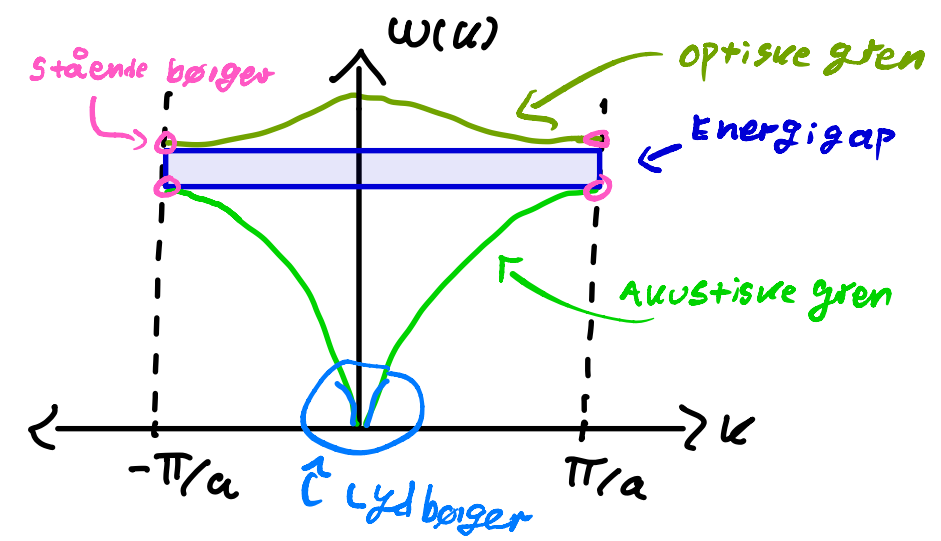
\includegraphics[width=0.5\textwidth]{bilder/sprednings_relasjon_diatomisk_kjede.png}}
    \label{fig:sprednings_relasjon_diatomisk_kjede}
    \caption{Spredningsrelasjonen for en diatomisk kjede}
\end{wrapfigure}
Hvis vi nå tegner $\omega(k)$ (\ref{fig:sprednings_relasjon_diatomisk_kjede}) vil de to løsningene være en optisk gren og en akustisk gren. Den øverste her er den optiske og den nederste er den akustiske. De nederste delene av den akustiske grenen tilsvarer lydbølger siden vi her har at gruppehastigheten er det samme som fasehastigheten. Det blå energigapet som er tegnet, kommer hvis $m \ne M$. Vi vil \underline{alltid} ha et slikt gap med mindre begge massene er helt like. I dette energigapet finnes det ingen løsninger. Derimot kan vi få stående bølger på ekstremalpunktene fordi man her vil ha at $\frac{\partial \omega}{\partial k} = v_g = 0$.

Det er også viktig å se på hvordan disse ser ut fysisk. Altså hvordan vil de akustiske og optiske grenene skille seg fysisk. Hvis man hadde hatt motsatt ladning på de to atomene ville det sett slik ut (\ref{fig:akustiske_og_optiske_fononer_diatomisk_kjede}):
\begin{figure}[H]
    \centering
    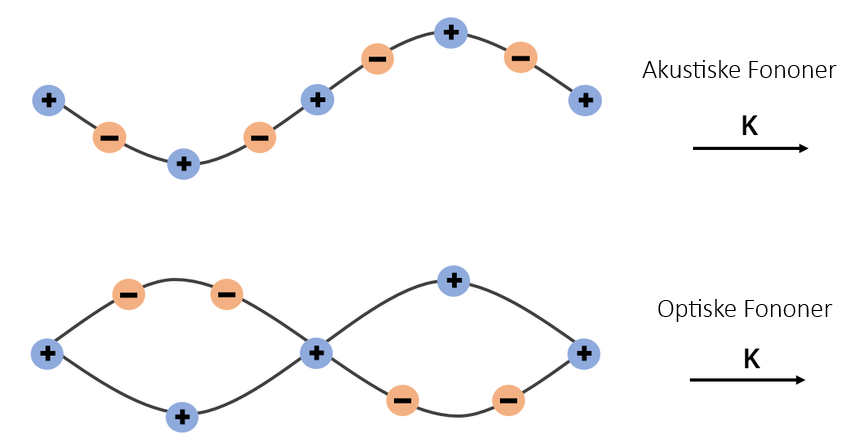
\includegraphics[width=0.5\linewidth]{bilder/akustiske_og_optiske_fononer_diatomisk_kjede.png}
    \caption{Akustiske og optiske fononer i en diatomisk kjede}
    \label{fig:akustiske_og_optiske_fononer_diatomisk_kjede}
\end{figure}
Altså ser vi at akustiske fononer beveger seg alle i samme retning, mens optiske fononer svinger fram og tilbake mellom hverandre. Dette siste bildet vil se annerledes i en dimensjon, hvor vi vil få langsgående komprimerende bølger som enten alle beveger seg i en stor kompresjonsbølge, eller mange med to og to atomer eller fler (avhengig av gitteret) som beveger fram og tilbake mellom hverandre. Altså blir optiske fononer mer koblet og mer intrikate og har derfor mer energi.

Noe som er nyttig å nevne nå er at fononene vil ha tre mulige polariseringer i hver mulig retning i tre dimensjoner. To tversgående(transversale) og en langsgående (longitudinal). Dette er i forhold til retningen vi beveger oss i. Altså vil langsgående bølger være bølger som er kompressjoner i samme retning som vi beveger oss i, mens tversgående bølger vil være forskyvninger normalt på impulsretningen. Altså kan vi bare ha kompresjoner på en måte, mens vi kan skape et normalplan på k, bestående av to basisvektorer som man kan ha oscillasjoner i som skaper de tversgående bølgene. Eksempler på tversgående bølger er lysbølger og vannbølger, mens en langsgående bølge kan være for eksempel lyd.

I et 3D-gitter med $s$ atomer i enhetscellen vil vi få 3 akustiske grener og $3s-3$ optiske grener. Totalt sett $3s$ grener. Disse grenene finnes som fire typer:
\begin{itemize}
    \item Langsgående Akustiske (LA)
    \item Tversgående Akustiske (TA)
    \item Langsgående Optiske (LO)
    \item Tversgående Optiske (TO)
\end{itemize}
For hver polariseringsmode vil vi få en optisk og en akustisk gren.

Noter også nå at vi for det meste ikke ser optiske fononer med mindre vi eksiterer dem selv. Slike kan eksiteres gjennom elektromagnetisk stråling som har samme energi som de tilsvarende optiske grenenergiene.

\delkapittel{Kvantisering av Fononer}
Vibrasjonene som skaper fononer er egentlig kvantiserte. Altså behandler vi faste stoffer som samlinger av veldig mange kvantemekaniske oscillatorer. Fononer er da de kvantiserte oscillasjonene. Vi har følgende for disse kvantiserte fononene:
\begin{equation}
    \omega = \sqrt{\frac{\gamma}{m}} \tab[2cm] E_n = (n + \frac{1}{2}) \hbar \omega
\end{equation}
Fononer og fotoner er bosonske eksitasjoner og har dermed ingen spinnstruktur og man kan ha uendelig mange av dem i samme kvantetilstand. Videre er fononer kvanta av et \enquote{vibrasjonsfelt} mens fotoner er kvanta av det elektromagnetiske feltet. Bølge-partikkel dualiteten gjelder for begge og vi har derfor for \enquote{partikkel}-\enquote{versjonene} av dem at $E = \hbar \omega, \vec{p} = \hbar \vec{k}$. Selv om vi derfor har en impuls hos fononer, er disse impulsene kun relative. Den fysiske impulsen i stoffet er fortsatt null og all lyd i stoffet er skapt av fononer som er relativ bevegelse inne i stoffet.

Vi kan også ha vekselvirkninger mellom fotoner og fononer som nevnt tidligere. Dette kan man man få til som alle andre vekselvirkninger, hvor energi og impuls er bevart. For å skape fononer fra fotoner og motsatt må da energien og impulsen deres være samme når man gjør en overgang. Altså må man ha noe som i dette bildet for spredningsrelasjonene deres.
\begin{figure}[H]
    \centering
    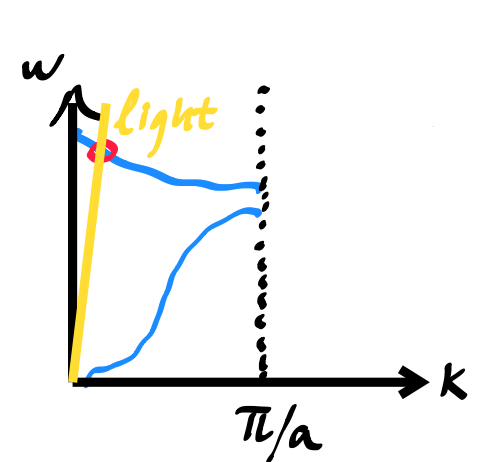
\includegraphics[width=0.3\linewidth]{bilder/lys_fonon_Vekselvirkninger.png}
    \caption{Lys-fonon vekselvirkninger}
    \label{lys_fonon_Vekselvirkninger}
\end{figure}
\nyside
\kapittel{Kapittel V: Fononer: Termiske egenskaper}
Det første vi vil ta for oss er varmekapasiteten til en gass av fononer, og dermed effektene av uharmoniske gittervekselvirkninger på fononene og krystallen.
\delkapittel{Fononets Varmekapasitet}
Med varmekapasitet mener vi varmekapasiteten ved et konsant volum. Dette er mer fundamentalt og mer relevant for oss enn varmekapasiteten ved konstant trykk. Denne varmekapasiteten er definert som:
\begin{equation}
    C_V \defeq \left(\frac{\partial U}{\partial T}\right)_V
\end{equation}
Hvor $U$ er energien og $T$ er temperaturen.

Bidraget fra fononene til varmekapasiteten til et krystrall kalles for gittervarmekapasiteten og er kalt $C_{\text{gitter}}$. Den totale energien til alle fononene ved en gitt temperatur i en krystall kan bli skrevet som en sum over alle impulser($K$) og polariseringer($p$):
\begin{equation}
    U_{\text{gitter}} = \sum_K \sum_p U_{K, p} = \sum_K \sum_p \underbrace{\braket{n_{K, p}}}_{\substack{\text{Termisk gjennomsnittlige antall}\\ \text{fononer i tilstand ($K, p$)}}} \hbar \omega_{K, p}
\end{equation}
Her modelleres dette gjennomsnittlige antallet gjennom Planck-fordelingen.
\seksjon{Planck-fordelingen}
Vi tar for oss en mengde identiske harmoniske oscillatorer i termisk likevekt. Antall oscillatorer i ($n+1$)-tilstanden i forhold til den $n$. tilstanden vil være:
\begin{equation}
    \frac{N_{n+1}}{N_n}= e^{-\frac{\hbar \omega}{k_B T}}
\end{equation}
på grunn av statistisk fysikk og da fra $N_n = e^{-\frac{E_n}{k_B T}}$. Vi får da at det gjennomsnittlige antallet tilstander i $n$ blir:
\begin{align}
    \braket{n} &=  \frac{\sum_x x \rho(x)}{\sum_x \rho (x)}\\
    &= \frac{\sum_n n e^{-n\frac{\hbar \omega}{k_B T} }}{\sum_n e^{-n\frac{\hbar \omega}{k_B T} }}
\end{align}
Ved å nå bruke ulike summerelasjoner kan vi finne at:
\begin{equation}
    \braket{n} = \frac{1}{e^{\frac{\hbar \omega}{k_B T}}-1}
\end{equation}
\seksjon{Finne varmekapasiteten}
Vi kan nå finne varmekapasiteten. Vi har da at:
\begin{equation}
    U = \sum_K \sum_p \frac{\hbar \omega_{K, p}}{e^{\frac{\hbar \omega_{K, p}}{k_B T}}-1}
\end{equation}
Her har vi såpass mange mulige verdier for $K$ at vi kan bytte om denne summen til et integral. Hvis vi nå da for hver polarisering har $D_p(\omega) d\omega$ antall moder på et lite intervall $d \omega$ vil vi si at $D_p(\omega)$ er tilstandstettheten vår. Altså hvor mange moder vi har per polarisering per omega. Vi får da:
\begin{equation}
    U = \sum_p \int d\omega D_p(\omega) \frac{\hbar \omega}{e^{\frac{\hbar \omega}{k_B T}} - 1}
\end{equation}
Vi gjør nå et lite variabelskifte ($x = \frac{\hbar \omega}{k_B T}$) og bruker at $C_{\text{gitter}} =  \left(\frac{\partial U}{\partial T}\right)_V$:
\begin{equation}
\label{eq:varmekapasitet_fononer_ferdig}
    \Rightarrow C_{\text{gitter}} = k_B \sum_p \int d\omega D_p(\omega) \frac{x^2e^x}{\left(e^x-1\right)^2}
\end{equation}
Vi har da funnet et utrykk for varmekapasiteten til fononene. Nå er det eneste spørsmålet hva $D_p(\omega)$ faktisk er.
\seksjon{Den Klassiske modellen (Dulong-Petit)}
Før vi ser på hvordan vi finner tilstandstetthetene er det greit med litt \enquote{historie}. I den klassiske modellen har vi som skrevet tidligere at:
\begin{equation}
    \label{eq:klassisk_energi_fononer}
    E = \frac{1}{2} m \vec{v}^2 + \frac{1}{2} \gamma \vec{r}^2
\end{equation}
Dette blir til 6 kvadratledd i energien, som ekvipartisjonsteoremet sier at gir oss $3 k_B T$ med termisk energi. For ett mol med oscillatorer har vi da at:
\begin{align}
    \braket{E} &= 3 N_A k_B T = 3 R T\\
    \Rightarrow C_V &=  \left(\frac{\partial U}{\partial T}\right)_V = 3 R
\end{align}
Altså har vi det som kalles for \underline{Dulong-Petit loven}. Denne loven fungerer bra ved høy temperatur, men er helt feil ved lav temperatur. Ved lav temperatur viser det seg at man får en $T^3$-avhengighet i varmekapasiteten. Dette kan vi tegne som:
\begin{figure}
    \centering
    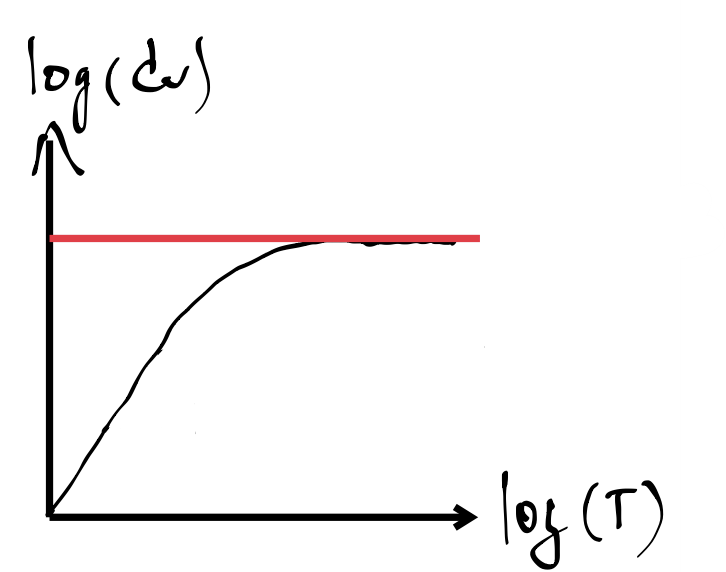
\includegraphics[width=0.5\linewidth]{bilder/dulong_petit_lov.png}
    \caption{Dulong-Petit loven mot data}
    \label{fig:dulong_petit_lov}
\end{figure}
Her er da den røde linjen Dulong-Petit loven, mens den svarte linjen er det man faktisk måler.
\seksjon{Semi-Kvantiserte modellen (Einstein)}
Einstein klarte å finne en bedre modell enn det over. Han brukte nesten samme ståsted som vi hadde øverst, med en liten forskjell. Istedenfor at vi tar hensyn til at vi kan ha forskjellige oscillatorer som tar del i varmekapasiteten som vi fant i likning (\ref{eq:varmekapasitet_fononer_ferdig}), så antok han at vi bare har en stor mengde med samme type oscillator. Altså vil i vår likning $D_p(\omega) = \delta(\omega - \omega_E) N$ for å få riktig antall oscillatorer ($N$) og kun en frekvens. Da får vi at:
\begin{align}
    C_{\text{gitter}} &= 3N \left(\frac{\hbar \omega_E}{k_B T}^2\right) \frac{e^{\frac{\hbar \omega_E}{k_B T}}}{\left(\frac{\hbar \omega_E}{k_B T} - 1\right)^2}
\end{align}
Denne fungerer mye bedre helt ned til en ganske så lav temperatur. Derimot fungerer den heller ikke ved en veldig lav temperatur. Dette er fordi vi her ikke har tatt hensyn til at vi kan ha mer enn en type oscillator og har antatt at alle har samme frekvens. Videre kommer 3-eren fra at vi har 3 dimensjoner
\delkapittel{Debye modellen}
La oss skrive opp resultatet vårt for varmekapasiteten igjen (\ref{eq:varmekapasitet_fononer_ferdig}):
\begin{equation}
    \Rightarrow C_{\text{gitter}} = k_B \sum_p \int d\omega D_p(\omega) \frac{x^2e^x}{\left(e^x-1\right)^2}
\end{equation}
Her vil vi i Debye modellen anta  at vi har en konstant lydhastighet for begge polariseringstypene, slik som det ville vært for et klassisk elastisk medie. Spredningsrelasjonen blir her da:
\begin{equation}
\label{eq:spredningsrelasjon_konstant_lydhastighet}
    \omega = v K
\end{equation}
Her er da $v$ en konstant lydhastighet. Vi må uansett finne ut av hva $D_p(\omega)$ er.
\seksjon{Tilstandstettheten i 3 dimensjoner}
Hvis vi ser på impulsrommet, vil vi finne et volum her som ser ut som: $V_{\text{impulsrommet}} = \frac{4}{3} \pi K^3$. Siden vi har løsninger i form av $K = \frac{2\pi}{L}$ vil vi få $N$ antall tilstander, hvor hver av disse tilstandene vil ta opp et volum av $_{\text{enhetscelle}} = \left(\frac{2 \pi}{L}\right)^3$:
\begin{align}
    N &= \frac{V_{\text{impulsrommet}}}{V_{\text{enhetscelle}}}\\
    &= \frac{\frac{4}{3} \pi K^3}{\left(\frac{2 \pi}{L}\right)^3} \\
\Rightarrow D(\omega) = \frac{dN}{d \omega} &=\frac{V K^2}{ 2 \pi^2} \frac{dK}{d\omega}
\label{eq:antall_tilstander_i_debye}
\end{align}
Ved å nå bruke \ref{eq:spredningsrelasjon_konstant_lydhastighet} får vi fort at:
\begin{equation}
    D(\omega) = \frac{V \omega^2}{2 \pi^2 v^3}
\end{equation}
Et viktig poeng her er at det kun vil være en viss mengde med bølgelengder man kan ta hensyn til i integralet. Siden vi ikke faktisk har et kontinuerlig stoff, men et diskret gitter av atomer, gir det ikke mening hvis bølgelengden til fononene er mindre enn det dobbelte av atomseparasjonslengden. Dette kan visualiseres slik:
\begin{figure}[H]
    \centering
    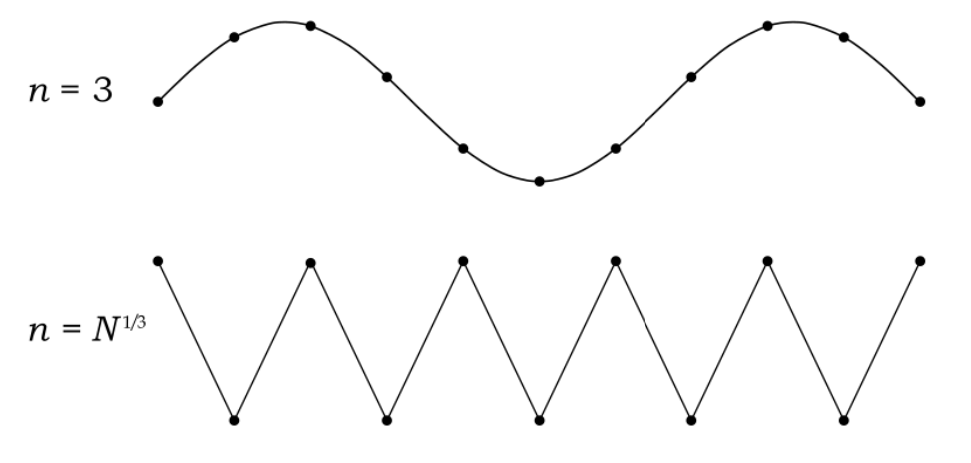
\includegraphics[width=0.5\linewidth]{bilder/debye_limit.png}
    \caption{Grensen til Debye modellen \cite{ShortDebye}}
    \label{fig:Debye_limit}
\end{figure}
Her ser vi hvordan atomene er ved ulike bølgelengder når bølgelengden er definert av:
\begin{equation}
    \lambda = \frac{2 L}{n}
\end{equation}
Altså blir den minste bølgelengden vi kan ha $\lambda_{\text{min}} = \frac{2 L}{\sqrt[3]{N}}$. Måten vi da ville funnet den høyeste gyldige frekvensen ved et viss antall atomer/primitive celler er ved å bruke likningen vår for N i \ref{eq:eq:antall_tilstander_i_debye}. Her kan vi løse likningen for N og finne ut at:
\begin{align}
    K^3 &= \frac{6 \pi^2 N}{V}
    \Rightarrow \omega_{\text{maks}} \defeq  \omega_{D}^3 = \frac{6 \pi^2 v^3 N}{V}
\end{align}
Altså blir det frekvensen på toppen av fermioverflaten. På en måte fermifrekvensen.

Som skrevet tidligere kan den termiske energien bli skrevet som:
\begin{equation}
    U = \int d\omega D(\omega) \braket{n(\omega)} \hbar \omega = \int_0^{\omega_D} d \omega \left( \frac{V \omega^2}{2 \pi^2 v^3}\right) \left(\frac{\hbar \omega}{e^{\frac{\hbar \omega}{k_B T}}-1}\right)
\end{equation}
for hver polariseringstype. Vi antar for simpelhet at alle disse er like så vi bare kan gange mer 3. Da får vi:
\begin{equation}
    U = \frac{3 V \hbar}{2\pi^2 v^3} \int^{\omega_D}_0 d \omega \frac{\omega^3}{e^{\frac{\hbar \omega}{k_B T}}-1} = \frac{3 V k_B^4 T^4}{2 \pi^2 v^3 \hbar^3} \int^{x_p}_0 dx \frac{x^3}{e^x - 1}
\end{equation}
Her har vi definert at $x = \frac{\hbar\omega}{k_B T}$. Vi har videre definert:
\begin{equation}
    x_D \defeq \frac{\hbar \omega_D}{k_B T} \defeq \frac{\Theta}{T}
\end{equation}
Hvor vi har definert \underline{Debye temperaturen $\Theta$}. Ved å sette inn utrykket for $\omega_D$ får vi dermed at:
\begin{equation}
    \Theta = \frac{\hbar v}{k_B} \left(\frac{6\pi^2 N}{V}\right)^{\frac{1}{3}}
\end{equation}
Da blir den totale energi til fononene:
\begin{equation}
    U = 9 N k_B T \left(\frac{T}{\Theta}\right)^3 \int^{x_D}_0 dx \frac{x^3}{e^x-1}
\end{equation}

Varmekapasiteten er da funnet ved å differensiere en av utrykkene for $U$. Vi kan dermed få at:
\begin{equation}
    C_V = 9 N k_B \left(\frac{T}{\Theta}\right)^3 \int_0^{x_D} dx \frac{x^4 e^x}{\left(e^x-1\right)^2}
\end{equation}
\seksjon{Debyes $T^3$-lov (veldig lave temperaturer)}
Ved veldig lave temperaturer vil et eventuelt bidrag fra alle frekvenser over $\omega_D$ ha mindre og mindre å si (dette kan vises). Altså kan vi integrere helt opp til uendelig ved slike lave temperaturer. Da kan vi løse integralet for $U$ analytisk:
\begin{equation}
    \int^\infty_0 dx \frac{x^3}{e^x-1} = \int^\infty_0 dx x^3 \sum^\infty_{s=1} e^{-sx} = 6 \sum_1^\infty \frac{1}{s^4} = \frac{\pi^4}{15}
\end{equation}
Som gir oss $U$ og $C_V$:
\begin{align}
    U &\approx \frac{3}{5} \pi^4 N k_B T \left(\frac{T}{\Theta}\right)^3 \\
    C_V &\approx \frac{12 \pi^4}{5} N k_B \left(\frac{T}{\Theta}\right)^3 
\end{align}
Hvor vi kan se at $C_V \propto T^3$. Dette er Debyes lov og passer veldig godt for stoffer ned til en veldig lav temperatur. Altså fungerer tilnærmingen bra når bare akustiske moder med lange bølgelengder er termisk eksitert. Disse er de modene som kan bli behandlet som et elastisk kontinuum med makroskopiske elastiske konstanter. Energien for modene med korte bølgelender er for høye for at de kan  bli eksitert i en stor nok grad ved disse lave temperaturene.

For krystaller er temperaturen man må ned til før denne loven gjelder ganske lov. Det kan faktisk være nødvendig å gå helt ned til $\Theta/50$ for å få en ren $T^3$ oppførsel.

Noe som kan være relevant nå er å se på hvordan de ulike modellene vi har sett på faktisk ser ut i impuls. Som vi så er Einsteins versjon kun en delta funksjon, mens Debyemodellen er lineær. Denne lineæriteten blir til $\omega^2$ når vi ser på $D(\omega)$. La oss derfor tegne disse to og et eksempel på eksperimentelle verdier man ser.
\begin{figure}[H]
    \centering
    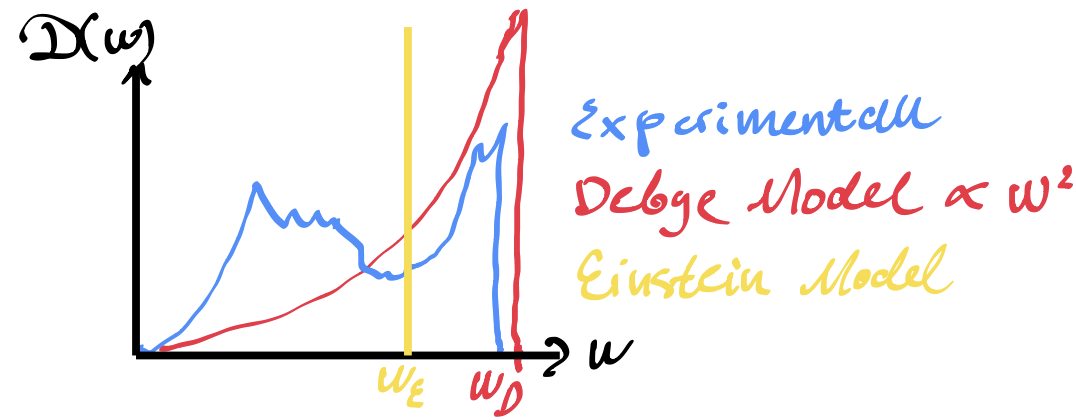
\includegraphics[width=0.5\linewidth]{bilder/tilstandstetthetssammenligning.png}
    \caption{Sammenligning av ulike tilstandstettheter}
    \label{fig:tilstandstetthetssammenligning}
\end{figure}
Her ser vi klart hvordan de ulike modellene skiller seg ut. Videre ser vi at Einsteins modell blir et slags snitt, mens Debye-modellen blir mye mer nøyaktig. Denne har også store problemer som man kan se, og er derfor ikke helt nøyaktig.

Noe annet å nevne som vi kan se er at modellene våre fungerer ganske bra. Vi har her bare tatt hensyn til fononer. Altså kan ikke elektroner bidra veldig mye til $C_V$ i seg selv. De bidrar faktisk bare med rundt 1\% av varmekapasiteten mens resten kommer fra fononene.
\delkapittel{Fermi-Dirac fordelingen}
Som vi har funnet ut vil vi få følgende energi i fermisfæren:
\begin{equation}
    E(n) = \frac{\hbar^2}{2m} \left(3 \pi^2 \frac{N}{V}\right)^{2/3}
\end{equation}
Dette gir oss at:
\begin{equation}
    N(E) = \frac{V}{3\pi^2} \left(\frac{2m}{\hbar} E\right)^{3/2}
\end{equation}
Tilstandsfordelingen blir da:
\begin{equation}
    g(E) = \frac{V}{2\pi^2} \left(\frac{2m}{\hbar}\right)^{3/2} \sqrt{E}
\end{equation}
Videre vil man dermed kunne regne ut forventningsverdien til antall tilstander ved en gitt energi. Eller da sannsynligheten for at en tilstand er okkupert. Altså har vi:
\begin{equation}
    \braket{n(E)}= g(E) \Delta E = k_B T g(E)
\end{equation}
Disse funksjonene kan tegnes på følgende måte:
\begin{figure}[H]
    \centering
    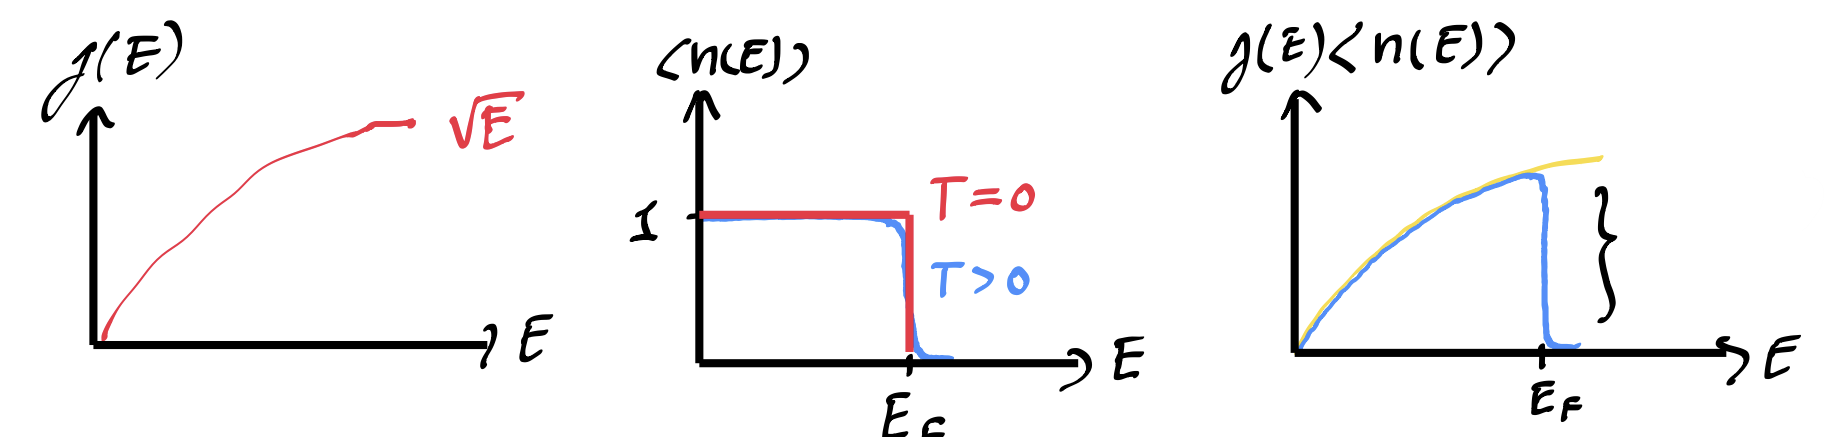
\includegraphics[width=1\linewidth]{bilder/fermi_dirac_fordelingen.png}
    \caption{Fermi-Dirac fordelingen}
    \label{fig:fermi_dirac_fordelingen}
\end{figure}
Vi ser dermed et viktig notat å merke seg: Sannsynligheten for at ferminivået er okkupert er alltid $50 \%$.
\delkapittel{Uharmoniske Krystallvekselvirkninger}
Teorien til gittervibrasjoner vi har diskutert så langt har vært begrenset i at den potensielle energien til gitterposisjonene er kun kvadratiske. Dette på grunn av fjærmodellen. Dette er en harmonisk teori. Konsekvenser av at vi har brukt denne teorien er:
\begin{itemize}
    \item To gittervibrasjoner vil ikke vekselvirke og en enkelt bølge vil ikke endre seg eller avta over tid.
    \item Det finnes ingen termisk utvidelse.
    \item De adiabatiske og isotermiske elastiske konstantene er like.
    \item De elastiske konstantene er uavhengige av trykk og temperatur.
    \item Varmekapasiteten blir konstant ved høye temperaturer $T > \Theta$
\end{itemize}
I ekte krystaller er ingen av disse punktene riktige på en god måte. Avvikene kommer av at vi ikke har noen anharmoniske ledd i energien (høyere enn kvadratiske ledd). Vi vil derfor diskutere noen enkle sider ved anharmoniske effekter.

Vakre demonstrasjoner av anharmoniske effekter er eksperimenter på vekselvirkninger mellom to fononer for å skape et tredje fonon slik at $\omega_1 + \omega_2 = \omega_3$. Altså at to fononer vil kunne klumpe seg sammen og bli til et nytt et. Slike tre-fonon prosesser har sitt opphav i tredje ordens ledd i gitterenergien. Dette er likt før høyere ordener. Alte blir fjerde ordens ledd til vekselvirkninger mellom 4 fononer.

\seksjon{Termisk Utvidelse}
Vi kan forstå termisk utvidelse ved å ta for oss den klassiske oscillatoren med to ekstra anharmoniske ledd. Vi antar at den potensielle energien på null temperatur er:
\begin{equation}
    U(x) = cx^2 - gx^3 -fx^4
\end{equation}
hvor alle konstantene er positive. $x^3$-leddet representerer asymmetrien til de gjensidige frastøtningene til atomene. $x-4$-leddet representerer mildningen til vibrasjonene ved store amplituder. Minimaet ved $x=0$ er ikke et absolutt minima, men er for små oscillasjoner en passende representasjon av et interatomisk potensial.

Vi regner ut gjennomsnittsforskyvningen i systemet ved å bruke Boltzmanns fordelingsfunksjon. Da har vi:
\begin{equation}
    \braket{x} = \frac{\int^\infty_\infty dx x e^{-\beta U(x)}}{\int^\infty_\infty dx e^{-\beta U(x)}}
\end{equation}
Hvis vi antar at de anharmoniske leddene i energien er små i forhold til den termiske energien $k_B T$ vil vi kunne få et svar for integralet her som gir oss:
\begin{equation}
    \braket{x} = \frac{3g}{4c^2} k_BT
\end{equation}
Her har vi forkastet f siden leddet vil ikke ha noe å si når $T \rightarrow 0$. Vi ser dermed at alle lengder vil forskyves. Denne faktoren kalles som oftes for $\alpha_L$. For generelle likninger av volumstørrelser kan man skrive:
\begin{align}
    L &\approx L_0(1 + \alpha_L T) \\
    V &\approx V_0(1 + \underbrace{\alpha_V}_{= \alpha_L / 3} T)
\end{align}
\delkapittel{Termisk Ledningsevne}
Den termiske ledningsevnekoeffisienten $K$ til et stoff er definert med hensyn til den stabile flyten av varme ned langs en stang med en temperaturgradient $\frac{dT}{dx}$:
\begin{equation}
    j_U = -K \frac{dT}{dx}
\end{equation}
Her er $j_U fluksen$ av termisk energi gjennom stangen. Siden vi har en gradient her og ikke bare forskjellen fra den ene siden av stangen og den andre, vil dette implisere at vi har en tilfeldig prosess og ikke en ren og direkte flyt fra den ene enden til den andre. Altså har vi tilfeldig bevegelse med mange kollisjoner gjennom stangen. Derfor vil den midlere frie veilengden komme i utrykket for den termiske fluksen $j_V$.

Fra kinetisk gassteori vil man kunne finne følgende utrykk for den termiske ledningsevnen:
\begin{equation}
    K = \frac{1}{3} C v l
\end{equation}
hvor $C$ er varmekapasiteten per volum, $v$ er snitthastigheten til partiklene og $l$ er den midlere frie veilengden. For fononene våre blir det da varmekapasiteten til fononene, hastigheten deres og deres midlere frie veilengde. Hastigheten her blir da lydhastigheten i et stoff. Typisk oppe i noen hundre meter per sekund.
\seksjon{Termiske Motstand til Fonongasser}
Den midlere frie veilengden til fononer er hovedsakelig bestemt av to prosesser. Geometrisk spredning og spredning av andre fononer. Som nevnt tidligere ville vi ikke ha slik spredning av andre fononer hvis vi ikke har noen anharmoniske ledd i energien. Det finnes derimot faktisk situasjoner hvor disse anharmoniske effektene dominerer.

Anharmoniske koblinger vil føre til at vi ikke lenger har rene fononer. Videre vil vi få en kobling mellom fononer som begrenser den midlere frie veilengden. Teorien til anharmoniske koblinger og termisk motstand forteller oss at $l \propto \frac{1}{T}$ ved høyere temperaturer. Dette kan bli forstått gjennom at antall eksiterte fononer er proposjonalt med $T$. Derfor burde spredningsfrekvensen være koblet til inversen av antall fononer som disse kan vekselvirke med.

For å kunne definere en termisk ledningsevne må det finnes mekanismer i krystallet som fører til at fordelingen av fononer i et lokalt område vil være i temrisk likevekt. Uten slike mekanismer kan vi ikke snakke om at den ene siden av stangen er ved en viss temperatur og den andre er i en annen viss temperatur.

Det er heller ikke nok å bare ha en måte å begrense den midlere frie veien, men det må også være mulig å skape en lokal termisk likevektsfordeling av fononer. Fononkollisjoner med en statisk uregelmessighet eller en krystallgrense i seg selv vil ikke etablere termisk likevekt siden slike kollisjoner ikke vil endre energien til individuelle fononer. 

\delseksjon{Tre-fononsprosesser uten termisk motstand}
Det er også ganske merkverdig at en tre-fononsprosess heller ikke vil gjøre dette. En slik prosess er definert av:
\begin{equation}
    \label{eq:trefononsprossess}
    K_1 + K_2 = K_3
\end{equation}
Dette er en ganske diskré effekt: den totale impulsen til fonongassen vil ikke endres av en slik kollisjon. En likevektsfordeling av fononer ved temperatur $T$ kan bevege seg nedover en krystall med en strømningshastighet som ikke er påvirket av slike tre-fononsprosesser i formen over \ref{eq:trefononsprossess}. For slike kollisjoner vil fononimpulsen $J$ være bevart:
\begin{equation}
    \vec{J} = \sum_{\vec{K}} n_{\vec{K}} \hbar \vec{K}
\end{equation}
Dette er fordi endringen i $\vec{J}$ vil være $\vec{K}_3 - \vec{K}_2 -\vec{K}_1 = 0$. Her er da $n_{\vec{K}}$ antall fononer med bølgevektor $K$.

For en fordeling hvor $\vec{J} \ne 0$, vil kollisjoner som \ref{eq:trefononsprossess}, ikke ha muligheten til å skape en komplett termisk likevekt siden de lar $\vec{J}$ forbli uendret.

\delseksjon{Tre-fononsprosesser med termisk motstand (Umklapp Prosesser)}
De viktige tre-fononsprosessene som skaper termisk motstand er ikke i formen $\vec{K}_1 + \vec{K}_2 = \vec{K}_3$ hvor $\vec{K}$ er bevart, men er derimot i formen:
\begin{equation}
    \vec{K}_1 + \vec{K}_2 = \vec{K}_3 + \vec{G}
\end{equation}
Hvor $\vec{G}$ er en resiprokal gittervektor. Disse prosessene kalles for \underline{umklapp prosesser}. Vi kan huske at $\vec{G}$ kan finne sted i alle impulsbevaringslover i krsystaller. I alle lovlige prosesser som beskrevet hittil, vil energi være bevart. Argumentet er som følger: de eneste meningsfulle fononimpulsene ligger i den første Brillouinsonen. Alle impulser som er lengre enn dette må bli flyttet tilbake igjen med en resiprokal gittervektor $\vec{G}$. Disse prosessene kalles også for U prosesser. 

En annen måte å si dette er: Ethvert punkt utenfor den første Brillouin-sonen kan uttrykkes som et punkt innenfor sonen. Bølgevektoren kan bli matematisk transformert til et punkt innenfor den første Brillouin-sonen gjennom en $\vec{G}$-vektor. Denne transformasjonen tillater spredningsprosesser som ellers ville brutt impulsbevaring: to bølgevektorer som peker mot høyre kan kombineres for å lage en bølgevektor som peker mot venstre. Dette fordi man da må ha en $\vec{G}$-vektor som drar den resulterende impulsen til venstre igjen. Altså: hvis $\vec{K}_1 + \vec{K}_2 = \vec{K}_3$ ikke er i den første Brillouinsonen, vil man måtte legge til en $\vec{G}$ som drar den tilbake igjen. Denne ikke-bevaringen av impuls er grunnen til at krystallimpuls ikke er ekte impuls.
\nyside
\kapittel{Kapittel VI: Fri elektrongass / Fermigass}
Vi kan forstå mange fysiske egenskaper til metaller, og ikke bare for enkle metaller, i forhold til den frie elektronmodellen. Ifølge denne modellen, blir valens-elektronene til de inneboende atomene i et stoff, ledningselektroner og kan bevege seg fritt gjennom volumet til metallet. Til og med i metaller hvor den frie elektrongassmodellen fungerer best, reflekterer ladningsfordelingen til ledningselektronene de sterke elektrostatiske potensialene til ionkjernen. Nytten til den frie elektromodellen er størst for egenskaper som mer eller mindre avhenger av de kinetiske egenskapene til ledningselektronene. Vekselvirkningene til ledningselektronene med ionene i gitteret vil bli sett på i \underline{neste} kapittel

De enkleste metallene er alkali-metallene: litium, sodium, potassium, cesium og rubidium. I et fritt elektron av sodium er valenselektronet i en 3s tilstand. I metallet blir dette elektron til et ledningselektron i 3s-ledningsbåndet.

En monovalent(et valenselektron) krystall som har N atomer, vil ha N ledningselektroner og N positive ionkjerner. 

Tolkningen av metallegenskapene i forhold til bevegelsen av frie elektroner ble utledet lenge før utviklingen av kvantemekanikk. Den klassiske teorien hadde flere oppsiktsvekkende suksesser. Spesielt utledning av Ohms lov og forholdene mellom den elektriske og termiske ledningsvnen. Den klassiske teorien derimot, mislykkes i å forklare varmekapasitet og den magnetiske mottakeligheten til ledningselektronene (Disse skyldes ikke feil i den frie elektronmodellen, men kommer av feil i den klassiske Maxwellfordelingen.)

Det er videre vanskeligheter med den klassiske modellen. For mange typer forsøk er det klart at et ledningselektron i et metall kan bevege seg fritt i en bane over flere atomiske avstander, uten å bli avsporet av kollisjoner med andre ledningselektroner eller atomkjerner. I en veldig ren prøve ved lave temperaturer, kan den midlere frie veien være mer enn en hel centimeter.

Hvorfor er kondensert materie så gjennomsiktig for ledningselektroner? Vel svaret på dette har to deler:
\begin{itemize}
    \item Et ledningselektron blir ikke avsporet av ionkjerner plassert på et periodisk gitter fordi materiebølger kan bevege seg fritt i en periodisk struktur på grunn av mattematikken vi snart vil utlede.
    \item Et ledningselektron er veldig sjeldent spredt av et annet et. Dette kommer av Paulis eksklusjonsprinsipp. ved en \text{fri elektrongass} mener vi en gass av frie elektroner som følger Pauli-prinsippet.
\end{itemize}
Denne klassiske modellen kalles for \underline{Drude}-modellen og beskriver en klassisk gass som følger Maxwell-Boltzmann statistikk. Den antar at elektronene mer eller mindre kolliderer med ionene på en klassisk måte over store avstander. altså tar den ikke hensyn til elektron-elektron vekselvirkninger eller mer enn det.
\delkapittel{Energinivåer i en dimensjon}
 Ta for deg en fri elektrongass. Vi vet at vi vil få følgende energi og løsning for Schrödingerlikningen:
 \begin{align}
     E &= \frac{\hbar^2 K^2}{2m} \\
     \psi(\vec{r}) &= \frac{1}{\sqrt{V}} e^{i \vec{k} \cdot \vec{r}}
 \end{align}
 Dette kommer fra å anta periodiske grensebetingelser og at $V = 0$. Vi får også en Fermi-sfære i impulsrommet definert av alle tilstandene vi har okkupert. For et atom kaller vi den øverste tilstanden for fermienergien $E_f$ og dermed vil fermienergien raskt bli:
 \begin{equation}
     E_F = \frac{\hbar^2 k_F^2}{2m}
 \end{equation}
 Spørsmålet er da: hva er fermi-impulsen. Vel det kan svares på raskt. I impulsrommet vil vi få som vi har gjort tidligere for å regne ut tilstandstettheten:
 \begin{equation}
     N = 2 \frac{\frac{4 \pi k_F^3}{3}}{(2 \pi / 3)^3}
 \end{equation}
 hvor vi her har ganget med 2 siden vi har 2 elektroner mer impulstilstand siden de kan ha motsatt spin. Altså to elektroner per orbital. Da kan vi raskt få at:
 \begin{equation}
     k_F = \left(\frac{3 \pi^2 N}{V}\right)^{\frac{1}{3}}
 \end{equation}

 
 som bare avhenger av partikkelkonsentrasjonen. NB!\ Her har vi antatt at alle elektronene er i de laveste mulige tilstandene. Altså at systemet er i grunntilstanden!

 Ved å sette inn dette i energien får vi at:
 \begin{equation}
     E_F = \frac{\hbar^2}{2m} \left(\frac{3 \pi^2 N}{V}\right)^{\frac{2}{3}}
 \end{equation}
Med dette kan vi finne tilstandstettheten til systemet (tilstander per energi). Den blir:
\begin{equation}
    D(E) = \frac{dN}{dE} = \frac{V}{2\pi^2} \cdot \left(\frac{2m}{\hbar^2}\right)^{\frac{3}{2}} \sqrt{E} = \frac{3N}{2E}
\end{equation}

\delkapittel{Varmekapasiteten til en Fri elektrongass}
Det spørsmålet som skapte de største vanskelighetene i den tidlige utviklingen av elektronteorien til metaller var varmekapasiteten til elektronene. Klassisk ville man tenkt at N valenselektroner ville ha en varmeenergi på $E_N = \frac{3}{2} N k_B T$. Eksperimentelt viste det seg ved romtemperatur at det faktisk var kun en hundredel av dette.

Dette enorme avviket distraherte mange av de som jobbet med dette først, slik som Lorentz: Hvordan kan elektronene delta i elektriske ledningsprosesser som om de er bevegelige, men ikke bidra til varmekapasiteten? Spørsmålet ble først svart på etter oppdagelsen av Paliprinsippet. Det viser seg at de eneste elektronene som kan bli termisk eksitert er de som er innen for en vidde av $k_BT$ unna fermienergien. Altså overflaten av fermisfæren. Dermed vil ikke alle $N$ eksiteres med en energi i orden $k_B T$ men kun en liten del i orden $T / T_F$. Dermed vil vi få at den totale elektronske termiske bevegelsesenergien $U$ er i orden:
\begin{equation}
    U_{\text{el}} \approx \frac{N T}{T_F} k_B T
\end{equation}
som gir oss en varmekapasitet:
\begin{equation}
    C_{\text{el}} = \frac{\partial U}{\partial T} \approx N k_B \frac{T}{T_F}
\end{equation}

Varmekapasiteten vil dermed som vi har nevnt tidligere være et bidrag fra fononer i orden $T^3$ og et bidrag fra elektroner i orden $T$.
En nøyere utregning gir:
\begin{equation}
\label{eq:termisk_varmekapasitet_fermigass}
    C_{\text{el}} = \frac{1}{2} \pi^2 N k_B \left(\frac{T}{T_F} \right)
\end{equation}

\delkapittel{Elektrisk ledningsevne og Ohms lov}
Impulsen til et fritt elektron er relatert til bølgevektoren gjennom $m \vec{v} = \hbar \vec{k}$. I et elektrisk felt $\vec{E}$ og et magnetisk felt $\vec{B}$ vil kraften $\vec{F}$ på et elektron beskrives av lorentz-kraften. Altså har vi at:
\begin{equation}
    \vec{F}= m \frac{d \vec{v}}{dt} = \hbar \frac{d \vec{k}}{dt} = -e \left(\vec{E} + \frac{1}{c} \vec{c} \times \vec{B}\right)
\end{equation}
Merk at likningen over er i CGS-enheter. Uten kollisjoner vil fermisfæren bevege seg i $\vec{k}$-rommet i en uniform hastighet av et konstant elektrisk felt. Vi integrerer likningen over med $\vec{B}= 0$, for å få $\vec{k}(t) - \vec{k}(0) = -\frac{e \vec{E} t }{}\hbar$.

Hvis kraften $\vec{F} = -e \vec{E}$ er påført ved $t = 0$ på en elektrongass som fyller fermisfæren i sentrum av impulsrommet, ved denne sfæren være forflyttet til et nytt sentrum av $\delta \vec{k} = - e \vec{E} t / \hbar$
Merk at fermisfæren er forflyttet som en hel enhet siden alle elektronene blir flyttet like mye.

På grunn av kollisjoner av elektroner med urenheter på grunn av gitterurenheter og fononer, vil den forflyttede sfæren være opprettholdt i en stabil tilstand i det elektriske feltet. Hvis kollisjonstilstanden til elektronene er $\tau$ er forflytningen til færmisfæren gitt av forrige ligning med $t = \tau$. Hastigheten er som normalt da gitt av $\delta \vec{k}/ m = -e \vec{E} \tau / m $. Hvis vi er i et konstant elektrisk felt $\vec{E}$ med n elektroner av ladning $q = -e$ per enhetsvolum, vil den elektriske strømningstettheten være:
\begin{equation}
    \vec{j} = n q \vec{v} = n e^2 \tau \vec{E} / m
\end{equation}
Dette er \underline{Ohms lov}.

Videre er den elektriske ledningsevnen definert av:
\begin{align}
    \vec{j} &= \sigma \vec{E}\\
    \Rightarrow \sigma &= \frac{ n e^2 \tau}{m}
\end{align}
Den elektriske mostanden er definert som inversen av dette og derfor:
\begin{equation}
    \rho = \frac{m}{ne^2\tau}
\end{equation}

\delseksjon{En viskøs bremsekraft}
Man kan også endre på hvordan frie elektroner beveger seg ved å legge til en slags bremsekraft. Altså kan vi gjøre noe som:
\begin{equation}
    F = m\frac{d v}{dt} = -e E - \Gamma v
\end{equation}
Dette vil gi en løsning for hastigheten i formen:
\begin{equation}
    v(t) = e^{- \Gamma t / m} - \underbrace{\frac{e}{\Gamma m} E}_{\text{Strømningshastighet}}
\end{equation}
Her vil elektroner fortsette å kollidere med fononer på grunn av gitterdefekter og urenheter. Ved å annerkjenne at $\Gamma = \frac{1}{\tau}$ vil vi da få en driftshastighet: $v_d = \frac{e \tau E}{m}$. Videre vil da elektronenes midlere frie veilengde bli til:
\begin{equation}
    l = v_F \tau
\end{equation}
For lave temperaturer vil vi ha få fononer og dermed få en enorm veilengde i en ballistisk skala.
\delkapittel{Bevegelse i magnetfelt}
La oss ta for oss det samme systemet med kollisjoner, men i et magnetisk felt. Altså har vi at:
\begin{equation}
    F = m \left(\frac{d}{dt} + \frac{1}{\tau}\right) = -e \left(\vec{E} + \frac{1}{c} \vec{v} \times \vec{B}\right)
\end{equation}
I en stabil tilstand i et statisk elektrisk felt vil alle de tidsderiverte være null. Da får vi en driftshastighet:
\begin{align}
    \label{eq:bevegelse_i_magnetfelt}
    v_x &= -\frac{e \tau}{m} E_x - \omega_c \tau v_y \\
    v_y &= -\frac{e \tau}{m} E_y + \omega_c \tau v_x \\
    v_z &= -\frac{e \tau}{m} E_z
\end{align}
Her er $\omega_c = \frac{e B}{m c}$ \underline{syklotron-frekvensen}
\seksjon{Hall effekten}
Hallfeltet er det elektriske feltet utviklet over to sideflater av en leder, i retning $\vec{j} \times \vec{B}$ når en strøm $\Vec{j}$ strømmer over et magnetisk felt $\vec{B}$. Vi kan se for oss en stang med et langsgående elektrisk felt $E_x$ og et tversgående magnetfelt. Hvis en strøm ikke kan flyte ut av stangen i y-retningen må vi ha at $\delta v_y = 0$. Fra likningene over \ref{eq:bevegelse_i_magnetfelt} er dette bare mulig hvis:
\begin{equation}
    E_y = - \omega_c \tau  E_x = - \frac{e B \tau}{mc} E_x
\end{equation}
Mengden definert av:
\begin{equation}
    \boxed{R_H = \frac{E_y}{j_x B}}
\end{equation}
kalles for \underline{Hall koeffisienten}. For å regne ut den i vår enkle model bruker vi Ohms lov fra tidligere og har da at $j_x = n e^2 \tau E_x / m$. Vi får da at:
\begin{equation}
    R_H = \frac{E_y}{j_x B} = -\frac{e B \tau E_x / mc}{n e^2 \tau E_x B / m} = -\frac{1}{n e c}
\end{equation}
Dette utrykket er negativt for frie elektroner siden $e$ er positiv av definisjon. Altså vil vi her få likningen:
\begin{equation}
    E_y = R_H B j_x
\end{equation}
som forteller oss at vi vil få et indusert elektrisk felt i y-retningen hvis vi har et slikt tversgående magnetfelt selv om vi bare egentlig har et ekstern elektrisk felt i x-retningen.

\delkapittel{Den Termiske ledningsevnen til Metaller}
I kapittel 5 fant vi et utrykk for den termiske ledningsevnen til partikler med hastighet $v$, varmekapasitet $C_v$ og midlere fri veilengde $l$:
\begin{equation}
    K = \frac{1}{3} Cvl
\end{equation}
Den termiske ledningsevnen til en fermigass følger fra varmekapasiteten vi skrev tidligere i \ref{eq:termisk_varmekapasitet_fermigass}, sammen med $E_F = \frac{1}{2} mv_F^2$:
\begin{equation}
    K_{\text{el}} = \frac{\pi^2}{3} \frac{n k_B^2 T}{m v_F^2} v_F l = \frac{\pi^2 n k_B^2 T \tau}{3m} 
\end{equation}
hvor vi brukte at $l = v_F \tau$. Vi sa tidligere at fononene skaper varmekapasiteten, men er det elektronene eller fononene som bærer størstedelen av varmestrømmen i et metall? I rene metaller er elektronbidraget dominerende ved alle temperaturer. I urene metaller eller i uordnede legeringer, er elektronets midlere frie veibane redusert av kollisjoner med urenheter. Da kan fononbidraget bli sammenlignet med elektronbidraget.
\seksjon{Forholdet av Termisk og Elektrisk ledningsevne}
\underline{Widermann-Franz loven} sier at for metaler ved ikke for lave temperaturer, vil forholdet mellom den termiske- og den elektriske ledningsevnen være proporsjonal med temperatur, hvor forholdskonstanten er uavhengig av hvilket metall det er. Dette var et viktig resultat i teorien til metaller og underbygget bildet av en elektrongass som bæreren av ladning og energi. Det kan bli forklart ved å bruke formelen for $\sigma$ fra tidligere og den vi nettopp fant for $K$:
\begin{equation}
    \frac{K}{\sigma} = \frac{\pi^2 k_B^2 T n \tau / 3m}{n e \tau^2 / m} = \frac{\pi^2}{3} \left(\frac{k_B}{e}\right)^2 T
\end{equation}
\underline{Lorentz tallet} $L$ er videre definert som:
\begin{equation}
    L = \frac{K}{\sigma T}
\end{equation}
Ifølge det vi fant over for forholdstallet får vi da at:
\begin{equation}
    L = \frac{\pi^2}{3} \left(\frac{k_B}{e}\right)^2 = 2.45 * 10^{-8} \text{watt-ohm / deg$^2$}
\end{equation}
Som hverken inneholder $n$ eller $m$. Eksperimentelle verdier av $L$ ved 0 grader celsius og 100 grader celsius passer bra med tallet over.
\nyside
\kapittel{Kapittel VII: Energibånd }
Den frie elektronmodelle ntil metaller gir oss godt innblikk i varmekapasiteten, den termiske ledningsevnen, den elektriske ledningsevnen og den magnetiske mottakeligheten og elektrodynamikken til medallen. Derimot mislykkes modellen i å hjelpe oss med andre store spørsmål: forskjelllen mellom metaller, halvmetaller, halvledere og isolatorer: positive verdier til Hall-koeffisienten, relasjonen av ledningselektroner til valenselektroner og mange transportegenskaper, spesielt magnetotransport. Vi trenger en mindre naiv teori, og heldigvis viser det seg at nesten alle enkle forsøk på å forbedre denne modellen vil forbedre modellen veldig.

Forskjellen mellom en god leder og en god isolator er slående. Ledningsevnen til en god leder og en god isolator kan ha en forskjell på hele 30 ordener. Forskjellen er faktisk i ordenen $\propto 10^{32}$.

Hvert faste stoff inneholder elektroner. Det viktige spørsmålet for elektrisk ledningsdevne er hvordan elektronene virker ved et utenforliggende elektrisk felt. Vi vil se at elektroner i krystaller vil legge seg i \underline{energibånd} skilt av energiregioner hvor ingen bølgelignende elektronorbitaler finnes. Slike \enquote{forbudte} regioner kalles for \underline{energigap} eller \underline{båndgap} og kommer av vekselvirkningene mellom ledningselektronene med ionkjernene til krystallene.

Krystallet oppfører seg som en isolator hvis de tillatte energibåndene er enten fylte eller tomme. Da kan ingen elektroner bevege seg i et elektrisk felt. Hvis et eller flere bånd er delvis fylt (mellom 10\% til 90\%) vil du ha et metall. Hvis ett eller to bånd er delvis fylt eller nesten tomme har man et halvmetall eller en halvleder.

For å forstå forskjellene mellom disse, må vi ta hensyn til periodisiteten til gitteret i den frie elektronmodellen. Muligheten for slike båndgap er da den viktigste nye egenskapen her.

Vi vil også se andre ganske spektakulære egenskaper til elektronene i krystaller. For eksempel vil de bevege seg gjennom elektriske og magnetiske felt som om de hadde en effektiv masse $m^{*}$ som kan være mindre eller større enn elektronmassen og til og med negativ. Elektroner i krystaller reagerer på anvendte felt som om de har negative eller positive ladninger, og her ligger forklaringen til de negative og positive verdiene til Hall-koeffisienten.

\delkapittel{Den nesten frie Elektronmodellen}
I den frie elektronmodellen fikk vi tillatte energiverdier kontinuerlige fra null til uendelig i formen:
\begin{equation}
    E_k = \frac{\hbar^2}{2m} \left(k_x^2 + k_y^2 + k_z^2\right)
\end{equation}
hvor vi med periodiske grensebetingelser har at:
\begin{equation}
    k_i = \frac{2 \pi n_i}{L}
\end{equation}
og bølgefunksjoner i formen:
\begin{equation}
    \psi_k(r) = e^{ikr}
\end{equation}
som representerer bevegende bølger som bærer impulsen $\vec{p} = \hbar \vec{k}$.

Båndstrukturen til en krystall kan ofte bli forklart av den nesten frie elektronmodellen hvor båndelektronene er behandlet av svake pertubasjoner fra det periodiske potensialet til ionkjernene. Denne modellene svarer nesten alle de kvalitative spørsmålene om oppførselen til elektroner i metaller.

Vi vet at Bragg-refleksjon er en karakteristisk egenskap til bølgeforplanting i krystaller. Bragg-refleksjon av elektronbølger i krystaller skaper energigap ( ved Bragg-refleksjon finnes ikke bølgelignende løsninger av Schrödingerlikningen. Dette kan visualiseres som følger:
\begin{figure}[H]
    \centering
    \includegraphics[width=0.5\linewidth]{bilder/båndgap.png}
    \caption{Båndgap}
    \label{fig:båndgap}
\end{figure}
Det kan finnes flere slike gap. I tillegg spiller posisjonen til fermienergien i metallet mye å si som nevnt tidligere gjennom at antall elektroner i orbitalene har mye å si. Derfor blir energigapene svært viktige for å bestemme om et fast stoff er en isolator eller en leder.

Vi forklarer fysisk opphavet til energigapene i det enkle problemet av et 1D-lineært gitter med gitterkonstant $a$. Vi vil få et energigap ved $k = \pm \pi/A$ som tegnet i figuren over \ref{fig:båndgap}. Bragg-betingelsen for refleksjon sier at $(\vec{k} + \vec{G})^2 = k^2$ som i en dimensjon med diffraksjon av en bølge med bølgevektor $\vec{k}$:
\begin{equation}
    k = \pm \frac{1}{2} G = \pm n \pi / a
\end{equation}
hvor $G = \frac{2\pi n}{a}$ er en resiprokal gittervektor og $n$ er et heltall. Den første refleksjonen og da energigapet kommer ved $k = \pm \pi/a$. Mellom disse verdiene er da den første Brillouinsonen til dette gitteret. Videre vil vi også få energigap ved de andre heltallsverdiene til $n$.

Bølgefunksjonene ved $k=\pm \pi/a$ er ikke de bevegende bølger til frie elektroner, beskrevet av $e^{i \pi x / a}$ og $e^{-i \pi x / a}$. Ved disse spesielle k-verdiene vil bølgefunksjonene være laget av like deler bølger som beveger seg til høyre og venstre. Når denne Bragg-refleksjonsbetingelsen $k = \pm \pi / a$ er tilfredsstilt vil en bølge som beveger seg til høyre bli Bragg-reflektert til å bevege seg mot venstre og motsatt. Hver følgende Bragg-refleksjon vil reversere bevegelsesretningen til en bølge. En bølge som hverken går til høyre eller til venstre er bare en stående bølge som ikke går noe sted.

Den tidsuavhengige tilstanden er representert av stående bølger. Vi kan skape to forskjellige stående bølger fra denne løsningen $e^{i \pm \pi x /a}$:
\begin{align}
    \psi(+) = e^{i \pi x / a} + e^{-i \pi x / a} = 2 \cos(2\pi x /a)\\
    \psi(+) = e^{i \pi x / a} - e^{-i \pi x / a} = 2i \sin(2\pi x /a)
\end{align}
Hvor pluss- og minustegnet betegner om de bytter fortegn når man bytter $x \rightarrow -x$. Begge disse er bygget opp av like deler av venstre- og høyrerettede bevegende bølger.

\seksjon{Opphavet til Energigapet}
De to løsningene $\psi(+)$ og $\psi(-)$ konsentrerer sammen elektroner på forskjellige områder og derfor vil de to elektronene ha forskjellige verdier for den potensielle energien i feltet til ionene i gitteret. Dette er opphavet til energigapet. Sannsynlighetstettheten til en slik partikkel er $\rho = |\psi|^2$. For en ren omreisende bølge $e^{ikx}$ må vi for bevaring av ladningstetthet ha at $\rho = 1$. Derimot er ikke ladningstetheten konstant for lineærkombinasjoner av planbølger. La oss ta for oss $+$ bølgen. Vi har her at:
\begin{equation}
    \rho(+) \propto \cos^2(\pi x / a)
\end{equation}
Denne funksjonen vil konsentrere sammen elektroner (negativ ladning) på de positive ionene sentrert ved $x = 0, a, 2a, \dots$ og så videre hvor den potensielle energien er lavest i gitteret. For å få et bilde av dette tegner vi følgende graf av $u(x)$ som er gitterpotensialet:
\begin{figure}[H]
    \centering
    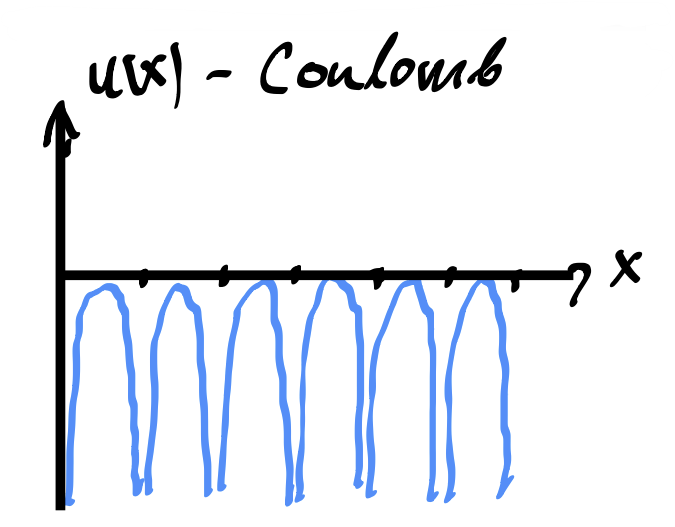
\includegraphics[width=0.5\linewidth]{bilder/gitterpotensialet_nestenfrimodell.png}
    \caption{Gitterpotensialet}
    \label{fig:gitterpotensialet_nestenfrimodell}
\end{figure}
HEr er da alle de merka punktene, heltallsmultipler av $a$. Dette er da posisjonene til ionkjernene.

Vi kan også tegne opp hvordan sannsynlighetstetthetene i de to tilfellene vil se ut:
\begin{figure}[H]
    \centering
    \includegraphics[width=0.5\linewidth]{bilder/sannsylighetstettheter_energibånd_1.png}
    \caption{Tegning av $u(x), \rho(+)$, og $\rho(-)$}
    \label{fig:sannsylighetstettheter_energibånd_1}
\end{figure}
Den negative løsningen vil være proporsjonal med sinus i annen istedenfor cosinus. Altså vil den da konsentrere elektroner vekk fra ionkjernene.

Når vi regner ut energien til disse to løsningene vil vi finne at energiforskjellen blir til $E_g$ som er det vi kaller \underline{båndgapsenergien}.

Merk at det er den løsningen som konsentrerer elektroner sammen vekk fra kjernene som har høyest energi!

Det vil også være nyttig å nå se på hva ulike ferminivåer tilsvarer av stoffer. Derfor tegner vi følgende figur:
\begin{figure}[H]
    \centering
    \includegraphics[width=0.5\linewidth]{bilder/femrinivåer_metall_halvleder_isolator.png}
    \caption{Forskjellige ferminivåer til ulike stoffer}
    \label{fig:femrinivåer_metall_halvleder_isolator}
\end{figure}
Her tilsvarer de røde linjene metaller. Altså får vi metaller hvis det er lett å eksitere fermielektronene til høyere energitilstander og dermed bevege seg som om de er i et ledningsbånd. Videre er den gule linjen hva ferminivået ville vært for halvledere. Her kan vi få to tilfeller for båndgapet. Enten er det større enn 3 eV eller mindre. Hvis det er større enn 3 eV har vi typisk isolatorer. Hvis båndgapet er mindre enn 3 eV har vi en halvleder. I dette tilfellet vil temperatur og andre effekter kunne eksitere elektroner enkelt nok over båndgapet slik at de kan bevege seg i et ledningsbånd.

\delkapittel{Bloch-funksjoner}
Felix Bloch fant ut i 1929 at løsninger av Schrödingerlikningen med et periodisk potensial må være av en spesiell form:
\begin{equation}
    \label{eq:blochs_teorem}
    \boxed{\psi_{\vec{k}}(\vec{r}) = u_{\vec{k}}(\vec{r}) = e^{i \vec{k} \cdot \vec{r}}}
\end{equation}
hvor $u_{\vec{k}}(\vec{r})$ har periodisiteten til krystallgiteret slik at $u(r + T) = u(r)$ hvor $T$ er en forskyvningsvektor til gitteret. Dette resultatet utrykker \underline{Blochs teorem}:
\begin{center}
\begin{adjustbox}{width=0.85\textwidth}
\parbox{\linewidth}{
Egenfunksjonene til bølgeligningen for et periodisk potensial er produktet av et planbølge $e^{i k r}$ multiplisert med en funksjon $u_k(r)$ med samme periodisitet somdet periodiske potensialet.
}
\end{adjustbox}
\end{center}
Et enkeltelektron i formen til likning \ref{eq:blochs_teorem} kalles for en Bloch funksjon og kan bli dekomponert i en sum av bevegende bølger, som vi vil se senere. Bloch-funksjoner kan bli samlet opp i bølgepakker som representerer elektroner som beveger seg fritt gjennom potensialfeltet til ionkjernene.

\delkapittel{Kronnig-Penney modellen}
Et potensial som kan bli løst analytisk er en lang rekke av firkantbrønner med høyde $U_0$ og bredde $b$. Da vil vi få brønner slik som tegnet her:
\begin{figure}[H]
    \centering
    \includegraphics[width=0.5\linewidth]{bilder/firkantbrønner.png}
    \caption{Firkantbrønner}
    \label{fig:firkantbrønner}
\end{figure}
I den første brønnen ved $0 < x < a$ hvor $U = 0$ vil vi ha bølger som er lineærkombinasjonen:
\begin{equation}
    \psi = Ae^{iKx} + Be^{-iKx}
\end{equation}
av planbølger som beveger seg til venstre og til høyre med fri energi. Videre vil de bølgene i regionen $-b < x < 0$ være en synkende løsning i formen:
\begin{equation}
    \psi = Ce^{Qx} + De^{-Qx}
\end{equation}
med potensialenergien minus den frie energien:
\begin{equation}
    E = U_0 - \frac{\hbar^2 Q^2}{2m} 
\end{equation}
Vi vil at den totale løsningen skal være i formen \ref{eq:blochs_teorem}. Da må følgende være sant:
\begin{equation}
    \label{eq:betingelse_firkantbrønner}
    \psi(a < x < a + b) = \psi(-b < x < 0)e^{ik(a+b)}
\end{equation}
Konstantene $A, B, C, D$ er da valgt så $\psi$ og $d\psi / dx$ er kontinuerlige ved $x = 0$ og ved $x = a$. Altså normale grensebetingelser for firkantbrønner. Ved $x = 0$, vil vi få ved å sammenlikne bølgefunksjonene at:
\begin{align}
    A + B &= C + D \\
    iK(A-B) &= Q(C-D)
\end{align}
For $x=a$, med å bruke \ref{eq:betingelse_firkantbrønner} for $\psi(a)$ under abrrieren i form av $\psi(-b)$ har vi at:
\begin{align}
    Ae^{iKa} + Be^{-iKa} = (Ce^{-Qb}+De^{Qb}) e^{ik(a+b)} \\
    iK(Ae^{iKa} - Be^{iKa}) = Q(Ce^{-Qb}-De^{Qb}) e^{ik(a+b)}
\end{align}
Disse likningene har kun en løsning hvis koeffisientene til $A,B,C,D$ forsvinner. Da får vi at:
\begin{equation}
    \left[\frac{Q^2-K^2}{2QK}\right] \sinh(Qb) \sin(Ka) + \cosh(Qb) \cos(Ka) = \cos(k(a+b))
\end{equation}
Som er ekkelt å regne ut. Dette er også et litt ekkelt resultat. Hvis vi antar at alle brønnene våre var deltabrønner tar vi grensene $b \rightarrow 0$ og $U_0 \rightarrow \infty$ slik at $\frac{Q^2 ba}{2}=P$. I denne grensen når $Q >> K$ og $Qb << 1$ får vi at likningen over reduseres til:
\begin{equation}
    \frac{P}{Ka} \sin(Ka) + \cos(Ka) = \cos(ka)
\end{equation}
Verdiene av $K$ hvor denne likningen har en løsning kan plottes som:
\begin{figure}[H]
    \centering
    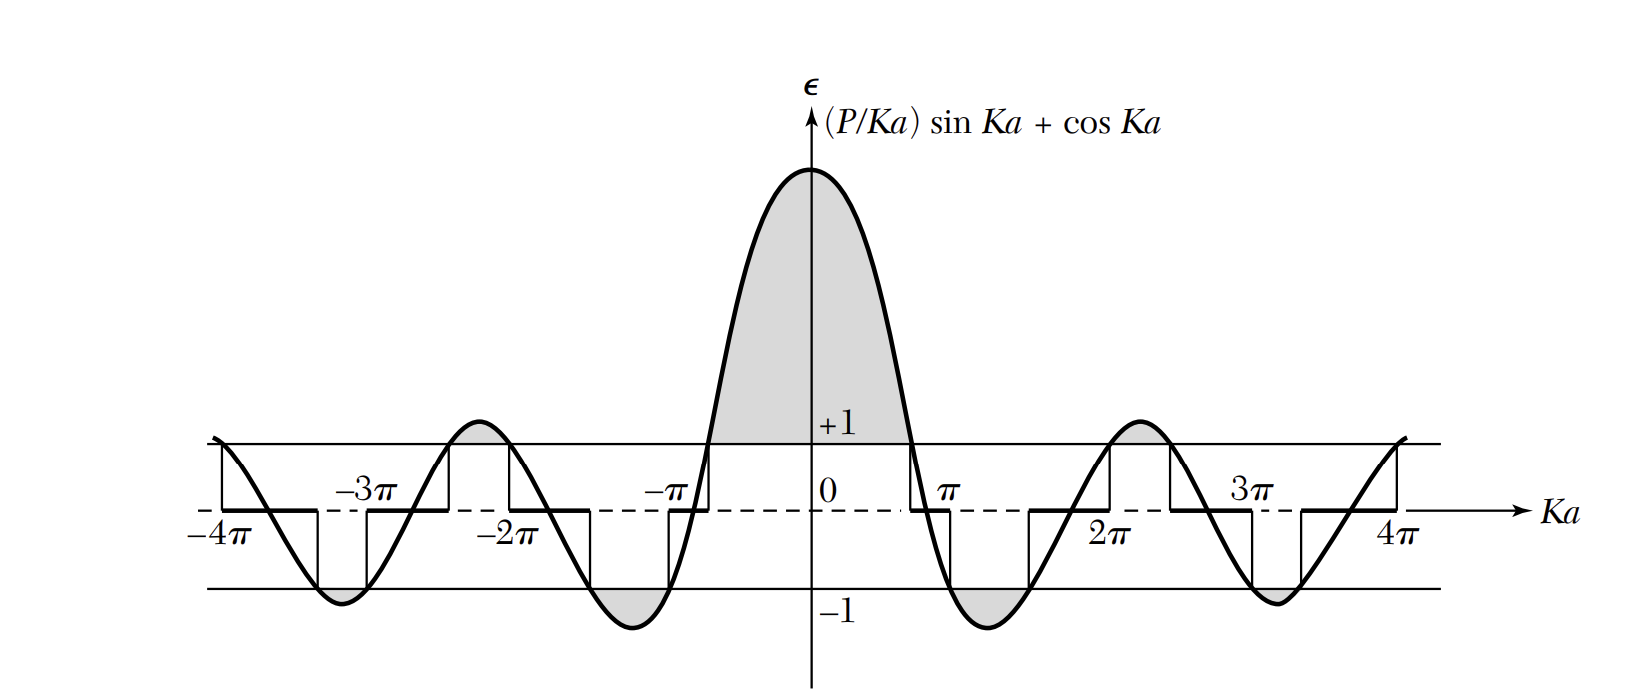
\includegraphics[width=0.5\linewidth]{bilder/energigap_kronigpenney_modellen.png}
    \caption{Energigap i Kronnig-Penney modellen}
\label{fig:energigap_kronigpenney_modellenl}
\end{figure}
Dette er plottet når $P = 3 \pi / 2$. Noter at venstresiden av likningen vi fant må være mellom $\pm 1$ for å følge likningen. Dette fordi høyresiden aldri kan bli større eller mindre en $\pm 1$ siden det bare er $\cos(x)$. Dermed får vi disse grå områdene i grafen over som representerer energigapene som ikke er lovlige. Her kan man også tegne hvordan energien vil se ut i forhold til $ka$. Man får da:
\begin{figure}[H]
    \centering
    \includegraphics[width=0.5\linewidth]{bilder/energibånd_i_kronig_penney_modellen.png}
    \caption{Energibåndene}
    \label{fig:energibånd_i_kronig_penney_modellen}
\end{figure}
Altså får vi som forventet, energigap ved $ka = n \pi$. Her har vi igjen at $ P = 3\pi / 2$.

\delkapittel{Bølgelikningen til et Elektron i et periodisk potensial (Sentrallikningen)}
Tidligere så vi for oss bølgelingningen ved en Brillouinsonegrense. Nå vi lvi se på bølgeligningen for et generelt potensial, ved generelle verdier for $k$. La $U(x)$ være et elektrons potensielle energi i et lineært gitter med gitterkonstant $a$. Vi vet at den potensielle energien er invariant under en krystallgitterforskyvning: $U(x) = U(x+a)$. En slik periodisk funksjon kan bli utvidet som en fourierrekke i de resiprokale gittervektorene $G$:
\begin{equation}
    U(x) = \sum_G U_G e^{i G x}
\end{equation}
Verdiene til koeffisientene $U_G$ for faktiske krystallpotensialer har en tendes til å minke raskts med økende magnitude av $G$. For et bart coloumb-potensial vil $U_G$ minke som $\propto\frac{1}{G^2}$.

Videre vil vi at den potensielle energien skal være en reell funksjon:
\begin{equation}
    U(x) = \sum_{G>0} U_G \left(e^{iGx} + e^{-iGx}\right) = 2 \sum_{G>0} U_G \cos (Gx)
\end{equation}
hvor vi har antatt for enkelthetsargumenter at krystallen er symmetrisk rundt $x= 0$ og at $U_0 = 0$.

Bølgelikningen til et elektron i krystallen er Schrödingerlikningen. Løsningene kalles egenfunksjoner eller orbitaler eller Bloch funksjoner. Eksplisitt ser bølgeligningen ut som:
\begin{equation}
    \left(\frac{1}{2m}p^2 + U(x)\right)\psi(x) = \left(\frac{1}{2m}p^2 + \sum_G U_G e^{iGx}\right) \psi(x) = \epsilon \psi(x)
\end{equation}
som antar at vi kun har ett elektron i gitterpotensialet og snittpotensialet til alle de andre ledningselektronene. Bølgelikningen $\psi(x)$ kan videre bli utrykt som en Fourier-rekke summet over alle lovlige bølgevektorer utrykket av grensebetingelsene slik at:
\begin{equation}
    \psi(x) = \sum_k C(k) e^{ikx}
\end{equation}
Hvor $k$er reell i formen $\frac{2\pi n}{L}$ siden disse verdiene tilfredsstiller periodiske grensebetingelser over lengden $L$.

Vi antar ikke og heller er det ikke sant at $\psi(x)$ er periodisk på nøyaktig samme måte som gitterperiodisiteten $a$. De bevegelige egenskapende til $\psi(x)$ er bestemt av Bloch-teoremet.

Videre vil ikke alle bølgevektorene i mengden beskrevet over ta del i Fourier-utviklingen til en Bloch-funksjon. Hvis utviklingen inneholder bølgevektoren $k$ er alle andre bidrag gitt av $k + nG$. Altså vil bidragene  kun komme fra en uendelig, men også uendelig mye mindre mengde av vektorer.

Ved å sette inn disse utviklingene inn i Schrödinger-likningen får vi:
\begin{equation}
    \sum_k \frac{\hbar^2}{2m} k^2 C(k) e^{ikx} + \sum_G \sum_k u_G C(K) e^{i(k+G)x} = \epsilon \sum_k C(k) e^{ikx}
\end{equation}
Siden hver eneste Fourier-komponent må ha samme koefissient på begge sider av likningen får vi \underline{Sentrallikningen}:
\begin{equation}
    \boxed{(\lambda_k - \epsilon)C(k) + \sum_G u_G C(k-G) = 0}
\end{equation}
med notasjonen:
\begin{equation}
    \lambda_k = \frac{\hbar^2 k^2}{2m}
\end{equation}
Denne formen av Schrödingerlikningen er en veldig nyttig form i et periodisk gitter, selv om den er helt uvant siden differensiallikningen har blitt byttet med mange algebraiske likninger. Mengden ser ekkel ut, siden det er uendelig mange verdier $C(k-G)$ man må finne ut av, men typisk er bare en veldig liten mengde nok for å se på det vi vil se på. Ofte så få som to eller fire.


% Forelesning {13.03.2024 10:15-12:00}
\seksjon{Oppsummering av Sentrallikningen}
Så langt har vi funnet at for frie elektroner så følger de følgende energirelasjon:
\begin{equation}
  \label{eq:energi_for_frie_elektroner}
  E_k = \frac{\hbar^2 k^2}{2m}
\end{equation}
Hvis vi plotter denne ser den ut som en parabol. Vi har funnet ut at i våre periodiske potensialer så kan vi finne energibåndgap, altså hakk i denne parabolen. Da bånd fra en y til en annen y, hvor vi ikke finner noen energier. Altså har vi ulovlige energibånd. Dette skaper ulike egenskaper i materialer % legg til mer info.

For et periodisk potensial fant vi at vi fikk Bragg spredning av elektronbølger. Videre fant vi også stående bølger i krystaller.

Vi fant også \underline{Block-Funksjonene}. Disse så generelt slik ut:
\begin{equation}
  \label{eq:block_funksjoner}
  \psi_{\vec{k}}(\vec{r}) = e^{i\vec{k}\cdot\vec{r}}u_k(\vec{r})
\end{equation}
Disse var da løsningene til Schrödingerlikningen med et periodisk potensial.
Videre ser Schrödinger likningen slik ut for et potensial:
\begin{align}
  \label{eq:schrödinger_likningen_med_periodisk_potensial}
  \left\{  -\frac{\hbar^2}{2m}\nabla^2 + u(\vec{r})  \right\}\psi(\vec{r}) = E\psi(\vec{r}) \\
  u(\vec{r}) = u(\vec{r} + \vec{R})
\end{align}
Altså blir potensialet her $\vec{R}$-periodisk. Ved å nå bruke foriertransformer så kan vi gjøre om denne differensiallikningen til en algebraisk likning. fouriertransformene er definert slik:
\begin{align}
  \psi(x) &= \sum_k c_k e^{ikx} \\
  u(x) &= \sum_G u_g e^{iGx}
\end{align}
Disse gir oss \enquote{sentrallikningen}:
\begin{equation}
  \label{eq:den_sentrale_likningen}
  \left(\frac{\hbar^2 k^2}{2m} - E\right)c_k + \sum_G u_g c_{k-G} = 0
\end{equation}
Denne likningen kobler hver ukjente koeffisient $c_k$ til et lite underset av alle andre $c_k$. Dette ser vi fra at $k$ er definert fra periodiske grensebetingelser som gir oss at $k = \frac{2\pi}{L}$, mens g er definert ut i fra krystallgitteret vårt. Altså: $G = \frac{2pi}{a}$. Siden $a >> L$ så blir stegene mellom $G$-ene enormt mye større enn de mellom $k$-ene. Da ser vi at vi har veldig mange flere $k$-er for hver $g$. Dermed kobles bare hver $c_k$ til et lite undersett av alle $k$-ene. Her blir da $G$-rommet et underrom av $k$-rommet.

Mer mattematisk så kobler for eksempel $c_{k_0}$ til $\{..., c_{k_0 - 2g}, c_{k_0 - g}, c_{k_0}, c_{k_0 + g}, c_{k_0 + 2g}\}$

\seksjon{Å Bevise Teoremet}
La oss nå anta at vi har en løsning til bølgefunksjonen $\psi(\vec{r})$.
Her kan vi da gjøre:
\begin{align}
  \psi(\vec{r}) &= \sum_{\vec{k}} c_{\vec{k}} e^{i \vec{k} {r}} \\
  \text{Gjennom sentrallikningen får vi:} \\
   \psi_k(\vec{r})&= \sum_{\vec{G}} c_{\vec{k} - \vec{G}} e^{i(\vec{k} - \vec{G}) 
   \vec{r}} \\
   &= e^{i\vec{k}\cdot\vec{r}} \sum_{\vec{G}}  c_{\vec{k} - \vec{G}}e^{-i \vec{G}\cdot\vec{R}}
\end{align}
Summen over $\vec{G}$ til slutt kan vi se at er $\vec{R}$ periodisk. Altså kunne vi ha kalt hele summen for en funksjon som er periodisk. Ved å sammenligne med definisjonen av Block-funksjonene, så har vi faktisk bevist at de er gyldige løsninger. Vi trenger bare å kalle summen for for $u(\vec{r})$ som vi brukte i definisjonen deres: 

\begin{equation}
  u_k(\vec{r}) = \sum_{\vec{G}} c_{\vec{k} - \vec{G}} e^{-i \vec{G} \cdot \vec{R}}
\end{equation}
\seksjon{Konsekvensene til Block's teorem}
Vi antar at vi har $\psi_{k'}(\vec{r})$ for en gitt $\vec{k'}$. Da kan vi skrive fra Block's teorem, at: $\psi_{k'}(\vec{r}) = e^{i\vec{k}\cdot\vec{r}} u_{k'}(\vec{r})$. Nå lar vi: $\vec{k} = \vec{k'} + \vec{G}$, hvor $\vec{G}$ er en resiprokalgittervektor. Nå kan vi da skrive:
\begin{align}
  \psi_k{\vec{r}} &= e^{i \vec{k} \cdot \vec{r}} e^{i \vec{G} \cdot \vec{r} u_{\vec{k} - \vec{G}}u(\vec{r})} \\
  &= e^{i\vec{k}\cdot\vec{r}}{u'}_{\vec{k}-\vec{g}}
\end{align}
Hvor: ${u'}_{\vec{k}-\vec{g}} = {u}_{\vec{k}-\vec{g}} e^{-i \vec{G}\cdot \vec{r}}$.
Denne nye Blockfunksjonen er \underline{like god} på alle måter som den originale. Konsekvensen her er at bølgevektoren $\vec{k}$ er vilkårlig med hensyn til addisjonen av en resiprokalgittervektor.

\delkapittel{Fyllingen av Elektronbåndene}
Fra de periodiske grensebetingelsene så får vi at: $\Delta k = \frac{2\pi}{L} = \frac{2\pi}{Na}$. Hvis vi nå sier at $\vec{k}$-verdiene innenfor  Brillouin-sonen (enhetscellen i k-rommet) $\left[-\frac{\pi}{a}, \frac{\pi}{a} \right]$, skaper et bånd, så ser vi at hvert bånd har N mulige k-verdier. Men hver av disse verdiene kan enten ha spin opp ($\uparrow$) eller ned ($\downarrow$). Altså har vi N tilstander per slikt bånd, med totalt 2N elektroner.

Hvis vi har \underline{et} valenselektron i hver primitive enhetscelle så vil materialet vårt være et \underline{metall}. Hvis det er \underline{to} valenselektroner per primitive enhetscelle så kan et bånd være helt fyllt, men ikke nødvendigvis. I 3 dimensjoner så kan båndene krysse over hverandre. Ved at disse båndene krysser hverandre mener jeg at: % fyll inn mer her.

\seksjon{Tomgitter Tilnærming}
I denne tilnærmingen lar vi potensialet $u \rightarrow 0$. Da blir alle Fourier-koeffisientene $u_g \rightarrow 0$. Konsekvensen her blir klart da at båndgapene forsvinner. Da blir sentrallikningen forenklet til at vi får frie elektroner igjen, som forventet. Det som er spennende å se på i denne frie modellen er hvordadan vi får energibånd får hver eneste $\vec{G}$. Dette er fordi alle løsninger med $\vec{k}$ vil også skape løsningene $\vec{k} + n \vec{G}, \tab[0.5cm] \vec{G} \in \mathbb{Z}$ Altså vil vi få veldig mange energinivåer: $E_n(\vec{k}) = \frac{\hbar^2(\vec{k} + \vec{G}_n)^2}{2m}$. Dette kan vi i se i bildet under:
\begin{figure}[h]
  \centering
  \caption{1D - Overlappende Tomgitter Tilnærming: \cite{WikipediaEN:Empty_lattice_approximation}}
  \includegraphics[scale=0.1]{bilder/1d_overlappende_tomgitter_tilnærming.png}
  \label{fig:1d_overlappende_tomgitter_tilnærming}
\end{figure}
%Forelesning 03.04.2024
\seksjon{Litt høyre potensial(fortsatt svakt)}

Fra kapittel 6 fant vi en dispersasjonsrelasjon for frie elektroner: $E = \frac{\hbar^2 k^2}{2m}$. I denne modellen så er alle materialer metaller siden vi alltid har et nytt nivå vi kan dytte elektroner opp i så de kan bevege seg "fritt". I kapittel 7 introduserte vi Bloch-funksjoner og fant ulike energibånd.
 I tillegg deriverte vi sentrallikningen: $\left(\frac{\hbar^2 k^2}{2m} - E\right) c_K + \sum_G u_G c_{k - G} = 0$. 

Videre så vi at i grensen $u_G \rightarrow 0$ så kunne disse parabolene overlappe slik som i figuren over i tomgittertilnærmingen \ref{fig:1d_overlappende_tomgitter_tilnærming}.

La oss nå øke potensialet (forstatt svakt) og anta at: $u(x) = 2 u_g cos(\frac{2\pi x}{G}) = \sum_G u_G e^{iGx}$, hvor $u_G$ er reell. Vi har også at $u_G = u_{-G}$ fra tidligere. Vi definerer nå at $u_g = u_{-g} = u$ hvor alle andre $u_G=0$. La oss nå se på sentrallikningen:
\begin{align}
  \left(\frac{\hbar^2 k^2}{2m} - E \right)c_k &+ \sum_G u_G c_{k-G} = 0 \\
  \left(\frac{\hbar^2 k^2}{2m} - E \right)c_k  &+ ... \\
  &+ u_{-2g} c_{k - (-2g)} \\
  &+ u_{-g} c_{k - (-g)} \\
  &+ u_{0} c_{k} \\
  &+ u_{g} c_{k - g} \\
  &+ u_{2g} c_{k - 2g}  = 0\\
\end{align}
Her kan vi simplifisere dette utrykket siden alt annet enn $u_g$ og $u_{-g}$ blir lik null siden vi antok det før vi begynte. Altså får vi:
\begin{align}
  \left(\frac{\hbar^2 k^2}{2m} - E \right)c_k  &+ ... \\
  &+ u_{-2g} c_{k - (-2g)} \\
  &+ u_{-g} c_{k - (-g)} \\
  &+ u_{0} c_{k} \\
  &+ u_{g} c_{k - g} \\
  &+ u_{2g} c_{k - 2g}  = 0 = \\
  \left(\frac{\hbar^2 k^2}{2m} - E \right)c_k  &+ ... \\
  &+ u_{-g} c_{k - (-g)} \\
  &+ u_{g} c_{k - g} = 0
\end{align}
Men nå vet vi jo at $k\rightarrow k-g$ også er en løsning. Altså gjelder også:
\begin{align}
  \left(\frac{\hbar^2 k^2}{2m} - E \right)c_k  &+ ... \\
  &+ u_{-g} c_{k - g - (-g)} \\
  &+ u_{g} c_{k - g - g} = 0
\end{align}
Videre så er jo også $k \rightarrow k+g$ og $k\rightarrow k+2g$ og så videre for evig. Vi kan få dette i matriseform. Vi skriver derfor at: $\lambda_k \defeq \frac{\hbar^2k^2}{2m}$ og får:
\begin{align}
  \begin{bmatrix}
    \lambda_{k-2g} - E& u_g & 0 & 0 & 0 \\
    u_g & \lambda_{k-g} - E & u_g & 0 & 0\\
   0 & u_g & \lambda_{k} - E &  u_g  & 0 \\
   0& 0 & u_g & \lambda_{k+g} - E& u_g  \\
   0& 0 & 0 & u_g & \lambda_{k+2g} - E  \\
  \end{bmatrix} \begin{bmatrix}
  c_{k-2g} \\
  c_{k - g} \\
  c_{k} \\
  c_{k+g}\\
  c_{k+2g}
  \end{bmatrix} = 0 \\
\Rightarrow \left | \begin{bmatrix}
    \lambda_{k-2g} - E& u_g & 0 & 0 & 0 \\
    u_g & \lambda_{k-g} - E & u_g & 0 & 0\\
   0 & u_g & \lambda_{k} - E &  u_g  & 0 \\
   0& 0 & u_g & \lambda_{k+g} - E& u_g  \\
   0& 0 & 0 & u_g & \lambda_{k+2g} - E  \\
  \end{bmatrix} \right | = 0
\end{align}
Vi kan trekke ut en mindre determinant av denne med dominante termer. Vi velger firkanten 11-22:
\begin{align}
  \left | \begin{bmatrix}
      u_g & \lambda_{k-g} - E & u_g\\
     u_g & \lambda_{k} - E &  u_g \\
    \end{bmatrix} \right | &= 0 \\
     \Rightarrow (\lambda_{k-g} - E)(\lambda_k - E) - u_g^2 &= 0 \\
     \Rightarrow E(k) &= \frac{1}{2}\left(\lambda_k + \lambda_{k-g}\right) \pm \left[\frac{1}{4}\left(\lambda_{k-g} - \lambda_k\right) +u_g^2 \right]^{\frac{1}{2}}
\end{align}

Ved å nå ta for oss sone-grensen $k=\frac{g}{2} = \frac{\pi}{a}$ så får vi at:
\begin{align}
  \lambda_k &= \frac{\hbar^2 k^2}{2m} = \frac{\hbar^2}{2m}\frac{g^2}{4} \\
  \lambda_{k-g} &= \frac{\hbar^2(k-g)^2}{2m} = \frac{\hbar^2 (\frac{g}{2}-g)^2}{2m} = \lambda_k \\
  \Rightarrow E(B.Z) = E\left(\frac{g}{2}\right) &= \lambda_{\frac{g}{2}} \pm u_g = \frac{\hbar^2 (\frac{1}{2}g)^2}{2m} \pm u_{1} = \underbrace{\frac{\hbar^2 \left(\frac{\pi}{a}\right)^2}{2m}}_{\text{Fritt elektron } E = \frac{\hbar^2 k^2}{2m}} \pm \underbrace{u_{1}}_{\text{Båndgap av størrelse } 2u_1}
\end{align}

Vi kan også vise at: 

A: $\psi_{k = \frac{g}{2}}(x) = e^{i g \frac{x}{2}} \pm e^{-ig\frac{x}{2}}$, som er en stående bølge. Se kapittel 7

B: $u_g = 0$, på grensen til B.Z-en

C: Nær nok grensen til B.Z-en så er båndstrukturen parabolsk.

\seksjon{Parabolske bånd}
For et fritt elektron hadde vi jo da: $E = \frac{\hbar^2 k^2}{2m}$, som er parabolsk, men hvordan gjør vi de andre elektronene parabolske også? Vel vi vil introdusere en effektiv masse $m^*$. Men hvorfor ville massen ha endret seg? Den vil endre seg fordi elektronet vil vekselvirke med omgivelsene (ionene rundt seg), og dermed vil bevegelsen dens være vanskeligere å idusere. Altså øker "treghetsmomentet" dens og dermed "massen" og den effektive massen.
\delseksjon{Krystall momentum}
$\vec{k}$ kan enten bli tolket som en bølgevektor eller som 3 kvantetall. $\hbar\vec{k}$ er \underline{ikke} det reelle/fysiske momentumet til elektronene. Vi har at $\hat{p} = -i \hbar \nabla$. For en Bloch-tilstand: $\psi_k(\vec{r}) = e^{i \vec{k} \cdot \vec{r}} u_k(\vec{r})$. La oss nå bruke $\hat{p}$ på denne:
\begin{align}
  \hat{p} \psi_k(\vec{r}) = -i \hbar \nabla \psi_k(\vec{r}) = \underbrace{\hbar \vec{k} \psi_K (\vec{r}) - e^{i \vec{k} \cdot \vec{r}} i \hbar \nabla u_k(\vec{r})}_{\text{Ingen skarp egenverdi}}
\end{align}
Selv om vi ikke har noen skarp egenverdi så er $\hbar \vec{k}$ fortsatt nyttig. Det er kalt krystall-momentum.
\delseksjon{Gruppehastighet og effektiv masse}
Vi husker at gruppehastighet er definert som: $v_g = \frac{d \omega(k)}{dk} = \frac{1}{\hbar} \frac{dE(k)}{dk}$.

Som gir oss aksellerasjonen: $a = \frac{d v_g}{dt} = \frac{1}{\hbar} \frac{d}{dt} \frac{dE(k)}{dk} = \frac{1}{\hbar}\left (\frac{d^2 E(k)}{dk^2} \frac{dk}{dt}\right)$.

Hvis vi nå ser på et eksternt felt fra newtons lov: $\hbar \frac{dk}{dt} = -e \varepsilon$

Som fører til at: $a = -\frac{1}{\hbar^2} \frac{d^2 E}{dk^2} e \varepsilon$.

Hvis vi nå definerer at $m^* = \left(\hbar^2 \frac{d^2 E}{dk^2}\right)^{-1}$ så får vi at $m^*a=-e\varepsilon$.

For frie elektroner blir jo da $m^* = m$, fra: $\frac{d^2 E}{dk^2} = \frac{d^2}{dk^2} \left(\frac{\hbar^2 k^2}{2m}\right) = \frac{\hbar^2}{m}$

%Forelesning 08.04.2024
\nyside
\kapittel{Kapittel VIII: Halvledere}
Ved null temperatur vil halvledere bli til insulatorer. Dette er fordi ved null temperatur vil et system ha falt ned i alle orbitalene så alle elektronene "sitter fast". Altså kreves det mye energi og et stort potensial over stoffet for å få til at elektroner hopper ut av disse orbitalene og begynner å bevege seg. 
Altså kan vi si for halvledere at:
\begin{itemize}
  \item Konduktivitet øker når temperatur øker. Dette blir da fordi fler elektroner eksiteres til ledningsbåndene eller nærmere dem ved en høyere temperatur. Da er det lettere å bevege dem og dermed har vi som sagt at konduktiviteten øker.
  
  NB!: I metaller vil en økende temperatur føre til mer og mer fononvekselsvirkninger som forstyrrer elektronene og dermed minker konduktiviteten.
  \item De har et båndgap på $\le 3 \text{eV}$.
  \item De har en ladningsbærerkonsentrasjon som er mye lavere enn for metaller. Altså har vi for metaller at $n \propto 10^{23} \ cm^{-3}$ elektroner, mens vi har opp til $n \propto 10^{13} \ cm^{-3}$ for halvlederen Germanium ved romtemperatur. Grunnen til at jeg spesifiserer romptemperatur er fordi metallene vil være fyllt opp med elektroner, mens de ikke er det for halvlederene. Altså vil antall elektroner i ledningsbåndene minke ved temperatur. Ladningsbærerkonsentrasjonen er jo da antall elektroner per volum i disse ledningsbåndene, og vil dermed også minke for halvledere ved lavere temperatur.
\end{itemize}
Nå definerer jeg at $n$ er antall elektroner i ledningsbåndene, mens $p$ er antall hull i valensbåndene. Da kan vi definere at:

En \underline{iboende} eller \underline{ren} halvleder har $n = p$:
\begin{itemize}
  \item En slik halvleder må være \underline{veldig} ren. Derfor blir de ofte bare av akademisk interesse.
\end{itemize}
På den motsatte siden har vi \underline{ytre} eller \underline{urene} halvledere, som har $n \ne p$:
\begin{itemize}
  \item Her har vi \underline{Doping}: "urene" og andre typer atomer i krystallstrukturen som har en tendens til å ta eller gi elektroner til omgivelsene.
\end{itemize}
Så kan vi tegne frie elektroner og elektroner i et periodisk potensial, i tillegg til hvordan elektronene ville vært fylt opp i disse i metaller i motsetning til halvledere eller insulatorer:

\begin{tikzpicture}
  \begin{axis}[
    axis lines = left,
    title = Frie Elektroner,
    xlabel = E,
    ylabel = D(E),
  ]
  \addplot[domain=0:5,color=black]{sqrt(x)};
  \end{axis}
\end{tikzpicture}
\hskip 5pt
\begin{tikzpicture}
  \begin{axis}[
    axis lines = left,
    title = Elektroner i periodisk potensial,
    xlabel = E,
    ylabel = D(E),
  ]
  \addplot[domain=0:2,color=black]{sqrt(x)};
  \addplot[mark=none, black] coordinates {(2,1.41421356237) (2,0)};
  \addplot[domain=2:3,color=black]{0};
  \addplot[mark=none, black] coordinates {(3,0) (3,1.73205080757)};
  \addplot[domain=3:5,color=black]{sqrt(x)};
  \end{axis}
\end{tikzpicture}
\hskip 5pt
\begin{tikzpicture}
  \begin{axis}[
    axis lines = left,
    title = Metaller (kapittel 7),
    xlabel = E,
    ylabel = D(E),
  ]
  \addplot[domain=0:2,color=black]{sqrt(x)};
  \addplot[mark=none, black] coordinates {(0.2,0.4472135955) (0,0)};
  \addplot[mark=none, black] coordinates {(0.4,0.63245553203) (0.2,0)};
  \addplot[mark=none, black] coordinates {(0.6,0.77459666924) (0.4,0)};
  \addplot[mark=none, black] coordinates {(0.8, 0.894427191) (0.6,0)};
  \addplot[mark=none, black] coordinates {(1, 1) (0.8,0)};
  \addplot[mark=none, black] coordinates {(1.2, 1.09544511501) (1,0)};
  \addplot[mark=none, black] coordinates {(2,1.41421356237) (2,0)};
  \addplot[domain=2:3,color=black]{0};
  \addplot[mark=none, black] coordinates {(3,0) (3,1.73205080757)};
  \addplot[domain=3:5,color=black]{sqrt(x)};
  \end{axis}
\end{tikzpicture}
\hskip 5pt
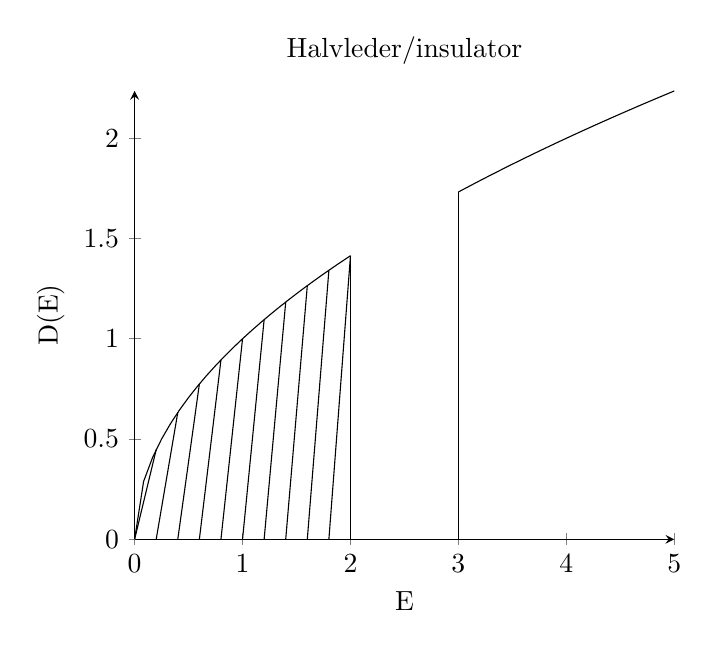
\begin{tikzpicture}
  \begin{axis}[
    axis lines = left,
    title = Halvleder/insulator,
    xlabel = E,
    ylabel = D(E),
  ]
  \addplot[domain=0:2,color=black]{sqrt(x)};
  \addplot[mark=none, black] coordinates {(0.2,0.4472135955) (0,0)};
  \addplot[mark=none, black] coordinates {(0.4,0.63245553203) (0.2,0)};
  \addplot[mark=none, black] coordinates {(0.6,0.77459666924) (0.4,0)};
  \addplot[mark=none, black] coordinates {(0.8, 0.894427191) (0.6,0)};
  \addplot[mark=none, black] coordinates {(1, 1) (0.8,0)};
  \addplot[mark=none, black] coordinates {(1.2, 1.09544511501) (1,0)};
  \addplot[mark=none, black] coordinates {(1.4, 1.18321595662) (1.2,0)};
  \addplot[mark=none, black] coordinates {(1.6, 1.26491106407) (1.4,0)};
  \addplot[mark=none, black] coordinates {(1.8, 1.3416407865) (1.6,0)};
  \addplot[mark=none, black] coordinates {(2, 1.41421356237) (1.8,0)};
  \addplot[mark=none, black] coordinates {(2, 1.41421356237) (2,0)};
  \addplot[domain=2:3,color=black]{0};
  \addplot[mark=none, black] coordinates {(3,0) (3,1.73205080757)};
  \addplot[domain=3:5,color=black]{sqrt(x)};
  \end{axis}
\end{tikzpicture}

% HER Videre har vi... (legg til mer her Sebastian)
Noter at det kjemiske potensialet $\mu$ vil være i midten av båndgapet.

\delkapittel{Hull}
Et hull er en ledig orbital ("tilstand") i et ellers fylt bånd. Det oppfører seg som en partikkel med motsatt ladning til elektronene i båndene. Den effektive massen til et slikt hull vil også være motsatt. Altså $m^{*}_h = -m_e^{*}$.

Fra før visste vi at effektiv masse $m^* \defeq \left(\hbar^2 \frac{d^2 E}{dk^2}\right)^{-1}$
Har vi huller i båndene våre kan elektronene bevege seg i motsatt retning i forhold til det man hadde forventet når man legger til et potnesial. Altås får man da en slags negativ effektive masse på elektronene, mens hullene får en positiv masse.

\seksjon{Båndstrukturen til GaAs og silikon}
\begin{tikzpicture}
  \begin{axis}[
    axis lines = left,
    title = Båndstukturen til GaAs,
    xlabel = k,
    ylabel = E,
  ]
  \addplot[domain=-5:5,color=black]{cosh(x / 2) + 3};
  \addplot[mark=none, black, dotted] coordinates {(-5,0) (5, 0)};
  \addplot[mark=none, red, dotted] coordinates {(-5,1.5) (5, 1.5)};
  \addplot[domain=-5:5,color=black]{-cosh(x / 2) - 4};
  \end{axis}
\end{tikzpicture}
\hskip 5pt
\begin{tikzpicture}
  \begin{axis}[
    axis lines = left,
    title = Båndstukturen til Silicon,
    xlabel = k,
    ylabel = E,
  ]
  \addplot[domain=-10:10,color=black]{cos(x / (2 * pi) * 360 / 2.25) * 10 + 20};
  \addplot[mark=none, black, dotted, thick] coordinates {(-10,0) (10, 0)};
  \addplot[mark=none, red, thick, dotted] coordinates {(-10,5) (10, 5)};
  \addplot[domain=-6:6,color=black]{-cosh(x / 3) * 8 - 10};
  \end{axis}
\end{tikzpicture}

Her blir båndet under valensbåndet og båndet over er ledningsbåndet. I tillegg representerer linjen i mitten energien $E = 0$, og den røde linjen er det kjemiske potensialet $\mu$. Vi ser også at fermi-fordelingen faller av fort. Altså er de mest mest interessante elektronene plassert på steder hvor vi har høyest aksellerasjon. På grafen til venstre har vi et direkte båndgap. Får å hoppe over må vi ha et foton med $E = E_g$ for å eksitere et elektron fra valensbåndet til ledningsbåndet. Energien her er neglisjerbar og er en vertikal prosess hvor elektroner hopper opp i energi med samme k.

I tillegg har vi her et \underline{Indirekte} båndgap på høyresiden fordi elektroner må endre k mer. Altså er "fononassistens" et krav og da er det mindre sannsynlig. Her til høyre får vi et båndgap på $E_g = 1.11 eV$. For å eksitere elektronene trenger de et foton med $E = E_g$, i tillegg ødelegger eller skaper man et fonon med $\Delta k$ krystall momentum for å få til eksitasjonen.


For solpaneler vil man ha et direkte båndgap som for eksempel GaAs fordi det bir bedre ytelse men der dyrere. Altså bruker satelitter GaAs mens hus bruker Si.

Videre vil jeg definere "Radierende Rekombinasjon":
\begin{itemize}
  \item Fotoner er emittert når elektroner går fra ledningsbåndet til valensbåndet.
  \item LED (light emitting diodes) (lys emitterende dioder)
\end{itemize}

Hvis vi ser på et foton som har lik energi som båndgapet har vi:
\begin{align}
  \hbar \omega_{optisk} = E_g \\
  \omega \propto \frac{E_g}{\hbar} \propto 10^{14} s^{-1} \\
  k_{optisk} = \frac{\omega_{optisk}}{c} \propto 10^6 m^{-1}
\end{align}
Sammenlign med $g_1 = \frac{2 \pi}{a} \propto 10^{10} m^{-1}$.

Altså ser vi at endringen man ville hatt i momentum ikke er i nærheten av nok til å komme seg ut av B.S-en. Altså er prosessen her en vertikal prosess til en veldig god approksimasjon. 

\seksjon{Å bruke absorbsjon til å forstå halvledere}
Vi kan bruke lys til å forstå halvledere. La oss se på hvor mye lys som er absorbert i forhold til energi:
\begin{tikzpicture}
  \centering
  \begin{axis}[
    axis lines = left,
    title = Lys absorbsjonn,
    xlabel = k,
    ylabel = E,
    width = 10cm,
    height = 7cm
  ]
  \addplot[domain=5:10, red]{3 / (1 + e^(-(x - 7.5)*1.5))};
  \addplot[domain=5:10, blue]{3 / (1 + e^(-(x - 8.5)*5))};
  \addplot[mark=none, black, dotted, thick] coordinates {(0,0) (0, 5)};
  \end{axis}
\end{tikzpicture}


Her er de to fargene direkte versus inderekte absorbsjon. Altså ser vi at de to tilfellene gir forskjellige grafer.
\begin{equation}
  I(\lambda) = I_0(\lambda) e^{-\mu (\lambda) s}
\end{equation}



% IVars notater
% Forelesning en eller annen gang



% Forelesning 15.04.2024
\delkapittel{Inneboende/Rene halvledere}
\delkapittel{Dopede/Urene halvledere}
Som vi har utledet i forrige delkappitel hadde vi at:
\begin{align}
  n &= \frac{1}{V} \int_{E_g}^{\infty} D_c(E) f_c(E, T)dE = \underbrace{\frac{1}{\sqrt{2}} \left( \frac{m_e^{*} k_B T}{\pi \hbar^2}\right)^{\frac{3}{2}} e^{-\frac{(E_g - \mu)}{k_B T}} }_{\propto 10^{25} m^{-3}\text{ for } T \approx T_{\text{romtemp}}} \\
  p &=\frac{1}{V} \int_{-\infty}^0 D_v(E) (1-f_e) dE = \frac{1}{\sqrt{2}} \left( \frac{m_h^{*} k_B T}{\pi \hbar^2}\right)^{\frac{3}{2}} e^{-\frac{\mu}{k_B T}}\\
  \Rightarrow np &= 4 \left(\frac{k_B T}{2 \pi \hbar^2}\right)^3 (m_e^{*} m_h^{*})^{\frac{3}{2}} e^{-\frac{E_g}{k_B T}}
\end{align}
Altså har vi ingen $\mu$-avhengighet. Ved inneboende halvledere har vi at $n=p$ (noter at np = konstant), som gir oss (ved å løse likningene over for $\mu$):
\begin{equation}
  \mu = \frac{E_g}{2} + \frac{3}{4} k_B T \ln{\left(\frac{m_h^{*}}{m_e^{*}}  \right)}
\end{equation}
Nå har vi da at dopede halvledere deles inn i to grupper. N og P-type.
\begin{itemize}
  \item N-Type:
  \begin{itemize}
    \item Det er donor-urenheter i dem. Altså atomer som vil donere vekk elektroner til omgivelsene.
    \item Ved å bruke Si og Ge så brukes oftest gruppe 5 elementer for å dope. Hovedbæreren i halvlederene er elektroner
  \end{itemize}
  \item P-Type: 
  \begin{itemize}
    \item Det er motager-urenheter. Altså atomer som gjerne tar imot elektroner fra omgivelsene.
    \item Igjen er det Si og Ge som brukes, men for å dope her bruker mann som oftest gruppe 3 elementer. Hovedbæreren i disse halvlederene er hull.
  \end{itemize}
\end{itemize}
Typiske tall her er da at man har mellom  0.0000001\% - 0.001\% med urenheter i et stoff. Å notere seg her er at Si har $5 * 10^{28}$ atomer per $m^3$, og en inneboende Ladningsbærerkonsentrasjon på $\approx 10^{16}$ per $m^3$ ved romtemperatur. Oppsummert kan vi da se at vi bruker elementer fra gruppe 4 som Si og Ge og doper dem med donorer eller motagere av elektroner fra gruppe 3 og 5. Slike små addisjoner av stoffer kan faktisk øke konduktiviteten til et stoff med hele 10 000x!

Denne dopingen gir nye tilstander i båndgapet og endrer det kjemiske potensialet. Disse ligger mellom ledningsbåndet og valensbåndet og for en n-type halvleder ligger den over, mens for en p-type halvleder ligger den under. Da flyttes det kjemiske potensialet fra halvveis til mellom disse donortilstandene og ledningsbåndet for n-type halvledere mens for p-type halvledere ligger de da nede mellom donortilstandene og  valensbåndet.

Ved en lav temperatur har man for donorer at $\mu$ må være mellom donortilstandene og lednignsbåndet. Ved en høyere temperatur vil alle donorelektroner gå i ledningsbåndet mens $\mu$ vil bevege seg mot $\frac{E_g}{2}$ fordi man da må ta elektroner fra valensbåndet for å eksitere dem til ledningsbåndet.
\kapittel{Kapittel IX: Nanoforskning}
Hvorfor er  folk så interesserte i nanoforskning? Vel. Vi kan begynne med å se på endelige faste stoffer (nano-strukturer). Når vi er i disse små skaalaene får vi kvanteinnesperring, endring av bulken, og vi har et stort overflateareal med reaksjoner.

Så langt i kurset har vi snakket om periodiske grensebetingelser. Vi har gjort dette for å fjerne alle overflateeffektene. Altså er vi uavhengige av hvor vi er på overflaten ved at vi har et potensial $u(x,y,z)=u(x+L,y+L,z+L)$. På grunn av disse periodiske grensebetingelsene får vi at momentumet til partikler i systemet er kvantiserte: $k = \frac{2 \pi}{a N} n$. Vi har også da at N atomer vil gi N normalmoder av vibrasjon. For lange men endelige kjeder vil tilstandstettheten være høy. Når vi har en film av tykkelse $d \propto \lambda$, vil vi ha kvanteeffekter gjennom dimensjonen til denne tykkelsen. Altså kan man få fripartikkelø tilstander langs den lengden som er veldig lang $k = \frac{2\pi}{\lambda}$, men kvantiserte tilstander langs den tynne lengden.

Områder man kan bruke dette er hvis man har en halvleder og et vakuum. Hvis man setter en tynn film over halvlederen, vil vi få en slags brønn i potensialet mellom halvlederen og vakuumet. Da kan vi gjøre en Ansatz: $\psi_{tot}(r) = \psi(z) \psi_{side}(x,y)$ hvor: $\psi(z) = Ae^{ik_z z}+Be^{-ik_z z}$. Hvis man da har en uendelig brønn, må bølgefunksjonen være null ved overgangen mellom disse tre stoffene. Da får vi det som kalles for en De-Broglie-betingelse: $2d = n\lambda \Rightarrow 2k_z d = 2\pi n$, som gir oss at:
\begin{equation}
  E_n = \frac{\hbar^2 k_z^2}{2m} = \frac{n^2 \pi^2 \hbar^2}{2m d^2}
\end{equation}

For en endelig brønn kan man vise at: $2k_z d + \Phi_i + \Phi_v = 2\pi n$.

\delkapittel{Kvantekorall}
En kvantekorall har en diameter på $\approx 70 Å$. Man før frie elektroner på overfaltten denne ligger på. Den er også bygget opp av cirka 50 jernatomer på en kobberoverflatefilm. Se bildet for hvordan de ser ut:
\begin{figure}[h]
  \centering
  \caption{Kvantekorallen}
  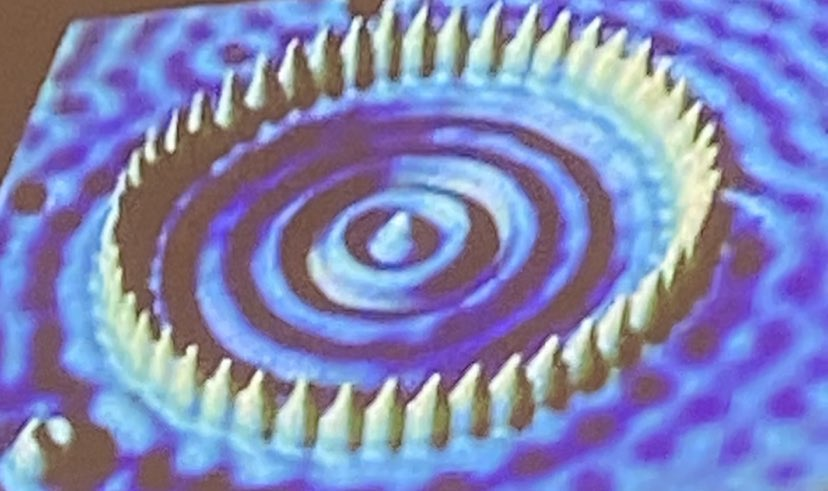
\includegraphics[scale=0.4]{bilder/kvantekorallen.jpg}
  \label{fig:kvantekorallen}
\end{figure}

Den letteste måten å modellere denne er ved å velge et potensial som er uendelig utenfor korallen og 0 innenfor. Altså blir dette en sfærisk uendelig brønn. Med dette potensialet får vi løsninger i formen til bessel-funksjonene: $\\psi_x(R) = AJ_m(kr) + \underbrace{BY_m(kr)}_{=0 \text{ fordi $Y_m$ divergerer når $r\rightarrow 0$}}$, med betingelsen $J_m(ka)$ og $\varepsilon = \frac{\hbar^2 \alpha*2}{2ma^2}$
\delkapittel{Halvleder-nanopartikler / Kvantepunkter ($r \le 100nm$)}
For å lage et elektron-hull par må du ha like mye energi som båndgapet i halvederen. I en halvleder nano-krystall vil vi få:
\begin{equation}
  E^{\text{nano}}_{\text{min}} = E_{\text{gap}} + \underbrace{ \frac{\hbar^2 \pi^2}{2 \mu r^2}}_{\substack{\text{Kvanteinnespering av elektronet og hullet} \\ \text{ som begge er lokalisert mer enn i bulken.}}} - \underbrace{\frac{1.8 e^2}{4 \pi \varepsilon_0 r}}_{\text{Coloumb-vekselsvirkning mellom hullet og elektronet}}
\end{equation}
Hvor her $\mu$ er den reduserte massen til elektronet og hullets effektive masser. Noter her også at det første leddet har med dreieimpulsen til dette paret å gjøre og avhenger av $1/r^2$. Disse kvantepunktene vil også endre på båndgapet. Jo mindre de er, jo større er båndgapet. I tillegg endrer jo da fargen til disse kvantepunktene seg til å bli blåere ved en høyere energi. Her kan man se kvanteeffektene i et bilde som viser slike kvantepunkter i et stoff preparert i ulike størrelser:
\begin{figure}[h]
  \centering
  \caption{Kvantepunktstoff}
  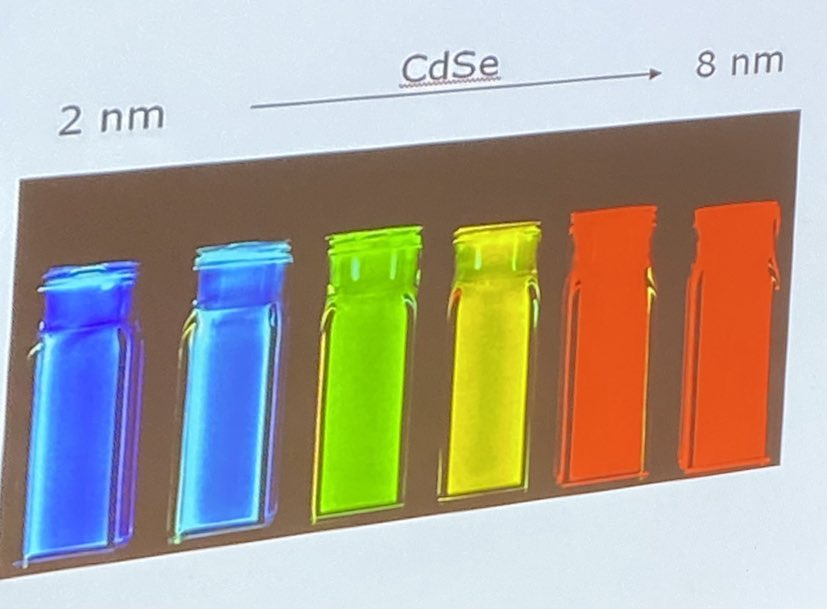
\includegraphics[scale=0.4]{bilder/kvantepunktstoff.jpg}
  \label{fig:kvantepunktstoff}
\end{figure}


\nyside
\printbibliography

\end{document}